% SD region of the Assignment 8 chapter (course Chapter 6): chapter head, overview, rows 1, 2, 3. Written Nov 17, 2026 from evidence 170-177
% and BD's 200-242. devopsDelivery.tex = this file + BD's devopsDelivery-bd.tex (rows 4-7) + devopsDelivery-sd-tail.tex (row 8).
% Section labels are fixed so both regions can cite each other. Times: New York (EST = UTC - 5 h); Jenkins and the server store UTC.
\chapter{Secure delivery and rollback}
\ChapterLabel{Delivery}
\index{delivery}\index{release}\index{rollback}

\paragraph{In one paragraph.} This chapter releases the course's small \emph{Startup Pricing Service} (Flask and Gunicorn; v1 charges USD~10 per unit, v2 USD~12)
on the Group~1 server through a secure pipeline \cite{DosManualV143}. Jenkins runs the tests on every pull request; for \texttt{main}, a trusted agent scans the dependencies and the source, builds \emph{one} image per reviewed commit,
scans it, pushes it to the Gitea container registry and records its digest; Ansible deploys that exact digest to \emph{staging}, and after a named person approves, the same digest to \emph{production}.
Every deployment is described by a \emph{release record} committed in Git, so a rollback re-applies an earlier record instead of rebuilding. Both releases (v1 on November~16 and v2 on November~17, 2026),
a production rollback from v2 to v1, a deliberately failed staging deployment and its recovery, a blocked scan and the monitoring view were run for real. SD owns rows 1, 2, 3 and 8 (application, image, Ansible,
diagram, release records and runbooks), BD rows 4 to 7 (Jenkins, scans and credentials, recoveries, monitoring). Grader access: the source is public at
\href{\GiteaRepoURL}{\texttt{group1-startup/twintrack}}; Jenkins pages behind the links below need a team account, so every number they show is also in the evidence listings of this chapter.

% ===== SD region: row 1 (10 points) =====
\section{The pricing service, its tests and locked inputs (10 points)}\label{Section:deliveryService}
\textbf{Owner:} SD. \textbf{Status:} v1 and v2 merged through reviewed pull requests and running as released images \StatusPass.

\paragraph{The service.} Three endpoints, from the course starter: \texttt{/} returns the service name, the version and the source commit; \texttt{/health} returns \texttt{ok} and the version; \texttt{/price?quantity=}$n$ returns
the total for $1 \le n \le 1000$ and HTTP~400 otherwise. v1 multiplies by 10, v2 by 12, so \texttt{quantity=3} gives 30 or 36 (\ListRef{DeliveryApp}). It keeps no state, which is why both environments and the rollback need no data plan.
The code entered \texttt{twintrack} through \href{\GiteaRepoURL/issues/11}{issue \#11} and \href{\GiteaRepoURL/pulls/12}{pull request \#12} (reviewed by BD, merge commit \href{\GiteaRepoURL/commit/12cdac7}{\texttt{12cdac7}}); v2 is a separate reviewed change,
\href{\GiteaRepoURL/pulls/21}{pull request \#21} (issue \#20, merge commit \href{\GiteaRepoURL/commit/06550eb4fe5d3315b31e1a1bd2fe1b4f034af77f}{\texttt{06550eb}}), identical to the course's v2: two constants and the expected totals in the tests.

\paragraph{Meaningful tests.} Four unit tests (\ListRef{DeliveryTests}): the price of 3 units through the function \emph{and} the HTTP endpoint; five invalid quantities (\texttt{0}, \texttt{-1}, \texttt{1001}, \texttt{abc}, \texttt{1.5}) must answer 400;
the release identity (\texttt{/} says the expected version, \texttt{/health} says \texttt{ok}); and a guard added by the team: the file \texttt{pricing-service/VERSION}, from which the pipeline names the release record, must equal the version
in \texttt{app.py}. They passed, a deliberately wrong expectation (31 instead of 30) failed with exit~1, and the restored file was identical to the starter (\ListRef{171}). The same tests run in the pipeline's first stage for every pull request and for \texttt{main}
(Section~\ref{Section:deliveryJenkins}); they are what makes a wrong price fail before an image exists.

\paragraph{Source identity.} The pipeline builds with \texttt{--build-arg APP\_COMMIT=}\emph{full commit}, the Dockerfile turns it into an environment variable, and \texttt{/} reports it. Ansible's last check compares the reported commit and version with the release record,
so a container that runs anything else fails the deployment. The public URLs report \texttt{975d13c\ldots} for v1 and reported \texttt{06550eb\ldots} for v2 (\ListRef{176}, \ListRef{230}, \ListRef{177}).

\paragraph{Locked build inputs.} \texttt{requirements.in} keeps the starter's ranges (Flask 3.1.x, Gunicorn 23.x). \texttt{pip-compile} 7.6.2 turned them into \texttt{requirements.txt} with exact versions and SHA-256 hashes for all 9 packages, direct and transitive (167 hashes);
recompiling gave the same packages and versions (\ListRef{172}). The image installs with \texttt{pip install --require-hashes --no-deps}, so a package that is not in the lock, or whose file differs, is refused.
The base image is pinned by digest, \texttt{python:3.13.18-slim-trixie@sha256:e48f59cd\ldots ed90} (the OCI index; its linux/amd64 manifest \texttt{48d88481\ldots} is recorded too), never by a moving tag \cite{DockerBuildBestPractices}.
pip-audit 2.10.1 found no known vulnerability in the lock at that time, which is not a claim that none exist (\ListRef{172}). After build \#6's image scan, BD's reviewed \href{\GiteaRepoURL/pulls/16}{pull request \#16} pinned the one OS package with a fix, \texttt{zlib1g}, to the exact tested version,
and removed \texttt{pip}, \texttt{setuptools} and \texttt{wheel} after the locked install (Section~\ref{Section:deliveryScans}); SD reviewed that the pin keeps the inputs locked: if Debian replaces that version, the build fails loudly and is fixed in a pull request.
The Dockerfile (\ListRef{DeliveryDockerfile}) also runs the service as UID 10001 with a health check; the Compose template adds a read-only root file system, \texttt{/tmp} as tmpfs, all capabilities dropped, no new privileges and 128~MiB of memory
\cite{DockerEngineSecurity,FlaskDeploying}. A local amd64 build of v1, which was never published, already answered correctly under those restrictions (\ListRef{173}).

\begin{longlisting}
\inputminted[fontsize=\scriptsize]{python}{config/twintrack/pricing-service/app.py}
\caption{\texttt{pricing-service/app.py} on \texttt{main} (v2; v1 differs only in \texttt{VERSION = "v1"} and \texttt{UNIT\_PRICE = 10}).}
\label{Listing:EDeliveryApp}
\end{longlisting}

\begin{longlisting}
\inputminted[fontsize=\scriptsize]{python}{config/twintrack/pricing-service/test_app.py}
\caption{\texttt{pricing-service/test\_app.py} on \texttt{main} (v2 expectations: version v2, total 36).}
\label{Listing:EDeliveryTests}
\end{longlisting}

\begin{longlisting}
\inputminted[fontsize=\scriptsize]{docker}{config/twintrack/pricing-service/Dockerfile}
\caption{\texttt{pricing-service/Dockerfile} on \texttt{main}: base image by digest, hashed install, pinned \texttt{zlib1g}, non-root user.}
\label{Listing:EDeliveryDockerfile}
\end{longlisting}

\begin{longlisting}
\inputminted[fontsize=\scriptsize]{text}{evidence/170-server-baseline-before-delivery-sd-2026-11-12.txt}
\caption{Read-only server baseline before any delivery work, November 12, 2026, 7:56~PM (real output).}
\label{Listing:E170}
\end{longlisting}

\begin{longlisting}
\inputminted[fontsize=\scriptsize]{text}{evidence/171-v1-unit-tests-pass-controlled-failure-restore-sd-2026-11-12.txt}
\caption{v1 tests: pass, a controlled failure, and the restore, November 12, 2026 (real output).}
\label{Listing:E171}
\end{longlisting}

\begin{longlisting}
\inputminted[fontsize=\scriptsize]{text}{evidence/172-locked-dependencies-base-image-digest-pip-audit-sd-2026-11-12.txt}
\caption{The lock with hashes, the base-image digests and pip-audit, November 12, 2026 (real output).}
\label{Listing:E172}
\end{longlisting}

\begin{longlisting}
\inputminted[fontsize=\scriptsize]{text}{evidence/173-v1-image-local-build-hardened-run-endpoint-checks-sd-2026-11-12.txt}
\caption{A local, unpublished v1 build run with the production restrictions; endpoint checks, November 12, 2026 (real output).}
\label{Listing:E173}
\end{longlisting}

% ===== SD region: row 2 (10 points) =====
\section{One image per reviewed commit, and the same digest promoted (10 points)}\label{Section:deliveryImage}
\textbf{Owner:} SD. \textbf{Status:} v1 (build \#7) and v2 (build \#11) each reached production with the digest that staging tested \StatusPass.

\paragraph{How an image is made and named.} Only the pipeline on \texttt{main} builds a release image, once per merged commit, tagged with the full commit and pushed to the Gitea registry as
\texttt{git.ssw590-g1.tech/group1-startup/pricing} \cite{GiteaContainerRegistry}. Right after the push the agent pulls the image back and reads its repository digest, which is the identity of the release from then on;
tags are only labels and are never deployed. The digest goes into \texttt{reports/digest.txt} and into the release records, and both Ansible runs of a build receive that same record, so staging and production cannot run different images
of the same release (Section~\ref{Section:deliveryJenkins} for the stages, \ListRef{216}).

\paragraph{Release records.} A release record is a small YAML file per release and environment (\texttt{releases/v1-staging.yml}, \ldots): digest, full commit, expected version and total, public URL, proxy network and, for production,
who approved and when. It holds metadata only. Jenkins writes and archives them; because \texttt{main} is protected they are committed afterwards through reviewed pull requests, byte-identical to the archived files
(SHA-256 compared; \href{\GiteaRepoURL/pulls/19}{pull request \#19} for v1, \href{\GiteaRepoURL/pulls/26}{pull request \#26} for v2; \ListRef{176}, \ListRef{177}). A change that touches \texttt{releases/} builds and deploys nothing (build \#9, \ListRef{223}).
The four records are in Section~\ref{Section:deliveryRecords}.

\paragraph{Traceability.} \ref{Table:DeliveryTrace} lists every build of \texttt{main} that reached the image stage. v1 and v2 each have one image, built once, scanned, tested in staging and promoted with the same digest.
Build \#8 shows the rule from the other side: merging a pipeline change produced a new image of the same v1, which staging ran but nobody promoted. The registry holds exactly the three pushed images (BD's reading of the package page, Section~\ref{Section:deliveryScans}; \FigRef{242}).

{\footnotesize
\begin{tabularx}{\linewidth}{L{1.2cm}L{1.3cm}L{2.75cm}YL{2.2cm}}
\caption{Traceability of the releases (Jenkins job \texttt{twintrack}, branch \texttt{main}; New York times)\label{Table:DeliveryTrace}}\\
\toprule \textbf{Build} & \textbf{Commit} & \textbf{Image digest} & \textbf{Scans, staging, approval, production} & \textbf{Evidence}\\ \midrule
\endfirsthead
\toprule \textbf{Build} & \textbf{Commit} & \textbf{Image digest} & \textbf{Scans, staging, approval, production} & \textbf{Evidence}\\ \midrule
\endhead \bottomrule \endlastfoot
\#6 (v1) & \href{\GiteaRepoURL/commit/49202f0}{\texttt{49202f0}} & none (not pushed) & tests, pip-audit and secret scan passed; image scan blocked: 53 HIGH, 0 CRITICAL; nothing deployed & \ListRef{213}\\
\#7 (v1) & \href{\GiteaRepoURL/commit/975d13c0c4cd3d0fab5035dd3d1817166bed8f07}{\texttt{975d13c}} & \texttt{sha256:}\newline\texttt{ce514106\ldots 98b2} & all scans passed (11 dated exceptions); staging v1, total 30, \texttt{changed=3}; approved by \texttt{brahmi} Nov~16, 11:36:33~PM; production same digest, v1, 30, \texttt{ok=9 failed=0} & \ListRef{216}, \ListRef{176}, \FigRef{217}\\
\#8 (v1) & \href{\GiteaRepoURL/commit/102da1d2e5a5d76d6de9cf6254f568b3b22b67d1}{\texttt{102da1d}} & \texttt{sha256:}\newline\texttt{5702d097\ldots 44ca} & scans passed; staging v1, 30; \textbf{rejected} at the approval by \texttt{brahmi}; production unchanged (``built and staged, not promoted'') & \ListRef{222}, \FigRef{221}, \ListRef{177}\\
\#11 (v2) & \href{\GiteaRepoURL/commit/06550eb4fe5d3315b31e1a1bd2fe1b4f034af77f}{\texttt{06550eb}} & \texttt{sha256:}\newline\texttt{ba2e211c\ldots f01c} & scans passed; staging v2, total 36; approved by \texttt{brahmi} Nov~17, 9:21:44~PM; production same digest, v2, 36; rolled back to v1 at 9:23:37~PM (Section~\ref{Section:deliveryRecovery}) & \ListRef{230}, \ListRef{231}, \FigRef{229}, \ListRef{177}\\
\#12 (fixture) & replay of \#11 & none (nothing built) & pip-audit exit 1 and secret scan exit 1 on a synthetic fixture; every later stage skipped & \ListRef{239}\\
\end{tabularx}
}
Builds \#5 (pip-audit could not write its cache, \ListRef{212}), \#9 (release records only) and \#10 (rollback file only) built no image. The full digests (\ListRef{177}):
{\footnotesize\begin{itemize}
\item v1, build \#7: \texttt{sha256:ce514106aead540576c4a9a67dd76e3a358547e5dcdf1be3c5057b82b92098b2}
\item build \#8: \texttt{sha256:5702d0975b2fcd510d642774f5d06d33a576307671d85f8d922ab90ac4fb44ca}
\item v2, build \#11: \texttt{sha256:ba2e211c8babc532913a9342325adbe5d897e4381aff560827f55b065d13f01c}
\end{itemize}}
Jenkins runs:
\href{https://ci.ssw590-g1.tech/job/twintrack/job/main/7/}{build \#7}, \href{https://ci.ssw590-g1.tech/job/twintrack/job/main/8/}{\#8}, \href{https://ci.ssw590-g1.tech/job/twintrack/job/main/11/}{\#11} (team sign-in required).

\paragraph{What is not claimed.} The images are not reproducible bit for bit: building the same commit again gives a new digest (build \#8 shows it), which is exactly why the digest, not the commit, is what gets promoted.
SD has no registry token, so the registry's own list is BD's screenshot (\FigRef{242}); SD checked the digests in Jenkins' archived reports and the identity through the public URLs.

\begin{longlisting}
\inputminted[fontsize=\scriptsize]{text}{evidence/176-v1-release-records-same-digest-staging-production-verified-sd-2026-11-16.txt}
\caption{Build \#7: the v1 digest, the two release records, their checksums against Jenkins, and SD's own HTTPS checks, November 16, 2026, about 11:55~PM (real output).}
\label{Listing:E176}
\end{longlisting}

\begin{longlisting}
\inputminted[fontsize=\scriptsize]{text}{evidence/177-v2-records-build-list-restore-run-recaps-traceability-final-state-sd-2026-11-17.txt}
\caption{Build lists of both jobs, the restore-run recaps, the build \#8 and v2 digests, the v2 records and the final public state, November 17, 2026, 11:34~PM (real output; read-only).}
\label{Listing:E177}
\end{longlisting}

% ===== SD region: row 3 (20 points) =====
\section{Ansible deployment, two environments and HTTPS (20 points)}\label{Section:deliveryAnsible}
\textbf{Owner:} SD. \textbf{Status:} every release and restore deployed by the playbook; unchanged second run shown on staging and production \StatusPass.

\paragraph{Tools and the path to the host.} ansible-core 2.22.0 on the trusted agent with the collection \texttt{community.docker} pinned to 5.4.0 (\texttt{ansible/requirements.yml}); the host meets both minimums (Python 3.9.25; Compose v5.6, where 2.18 is needed);
the playbook passed a syntax check and its template rendered into a Compose file that Compose accepted (\ListRef{174}) \cite{AnsibleGettingStarted}. Ansible connects as the account \texttt{deploy} with a key held only by Jenkins and uses \texttt{become}
for root \cite{AnsibleBecome}; that \texttt{sudo} and Docker access amount to host administration, which is written down as a risk (Section~\ref{Section:deliveryScans}). The server cannot reach its own Elastic IP on port~22 through the security group, so the agent reaches
\texttt{sshd} over the Docker bridge under the name \texttt{deploy-target}; \texttt{HostKeyAlias} and the committed \texttt{ansible/known\_hosts} make OpenSSH verify the same ED25519 key that has been pinned since Chapter~\ref{Chapter:Gitea}
(\texttt{SHA256:sJSqc\ldots}; \ListRef{175}, \ListRef{201}). The inventory holds no secret (\ListRef{DeliveryInventory}).

\paragraph{What the playbook does.} \texttt{ansible/deploy.yml} (\ListRef{DeliveryPlaybook}) takes one release record as variables and (1) checks it (environment name, \texttt{@sha256:} digest, version, total, \texttt{https://} URL);
(2) creates \texttt{/opt/startup/pricing-}\emph{env}; (3) renders the Compose file from the template (\ListRef{DeliveryTemplate}); (4) converges the Compose project \texttt{pricing-}\emph{env} with \texttt{build: never} and \texttt{pull: missing}, so the host can only
pull the named digest and never builds; (5) waits until \texttt{/health} answers \texttt{ok} \emph{through the public HTTPS name with certificate validation}; and (6) asserts that \texttt{/} reports the record's version and commit and that \texttt{/price?quantity=3}
gives the record's total. A record that names a missing image fails at step~4 (BD's staging failure, \ListRef{237}); a container that answers with the wrong version or price fails at step~6.

\paragraph{Environment separation.}
\begin{tabularx}{\linewidth}{L{3.0cm}YY}
\caption{Staging and production on the same host\label{Table:DeliveryEnvs}}\\
\toprule & \textbf{Staging} & \textbf{Production}\\ \midrule
\endfirsthead
\toprule & \textbf{Staging} & \textbf{Production}\\ \midrule
\endhead \bottomrule \endlastfoot
Public URL & \href{https://staging.ssw590-g1.tech/health}{\texttt{staging.ssw590-g1.tech}} & \href{https://app.ssw590-g1.tech/health}{\texttt{app.ssw590-g1.tech}}\\
Compose project and folder & \texttt{pricing-staging},\newline \texttt{/opt/startup/}\newline\texttt{pricing-staging} & \texttt{pricing-production},\newline \texttt{/opt/startup/}\newline\texttt{pricing-production}\\
Name on \texttt{gitea\_web} & \texttt{pricing-staging:8000} & \texttt{pricing-production:8000}\\
Release record & \texttt{releases/v}$n$\texttt{-staging.yml} & \texttt{releases/v}$n$\texttt{-production.yml} (with the approval)\\
Who deploys & the pipeline for every \texttt{main} build with an image; the \texttt{rollback} job without approval & only after the named approval (\texttt{brahmi} or \texttt{sakshi}), in the pipeline or the \texttt{rollback} job\\
Monitored & no (on purpose, Section~\ref{Section:deliveryMonitoring}) & Blackbox probe of \texttt{/health} every 30~s\\
\end{tabularx}
Neither container publishes a port: Caddy, the only service on 80 and 443, routes each name to its alias (BD applied SD's two blocks; certificates from Let's Encrypt, \ListRef{208}). A failed staging deployment stops the pipeline before the approval, so production is never touched by it.
Both share the host, Docker and the network, which is the single-server limitation (Section~\ref{Section:deliveryManual}).

\paragraph{Valid HTTPS.} The playbook's own checks run with \texttt{validate\_certs: true} and went through the public names in every successful run; SD's checks from outside used curl with certificate verification, and both URLs answered with HTTP~200 and a verified certificate
(\texttt{ssl\_verify=0} in \ListRef{176} and \ListRef{177}).

\paragraph{Runs and the unchanged second run.} The first deployment of each environment (build \#7) changed three tasks: the folder, the Compose file and the container (\texttt{ok=9 changed=3 failed=0}, \ListRef{176}). Idempotence was shown with the \texttt{rollback} job,
which runs the same playbook with a committed record and no rebuild (\ListRef{177}, BD's \ListRef{228}):
\begin{itemize}
\item rollback build \#5, \texttt{releases/v1-staging.yml}, Nov~17, 9:09~PM: \texttt{ok=9 changed=2} (staging was on build \#8's image, so the Compose file and the container moved back to the v1 digest);
\item rollback build \#6, the \emph{same} record, 9:12~PM: \texttt{ok=9 changed=0}, nothing reported as changed and the container was not restarted;
\item rollback build \#7, \texttt{releases/v1-production.yml}, approved by \texttt{brahmi}, 9:15~PM: \texttt{ok=9 changed=0} (production had run this record since build \#7).
\end{itemize}
Every check task is \texttt{changed\_when: false}, so \texttt{changed=0} really means that the desired state was already in place, not that the checks were skipped: they ran and passed each time.

\begin{longlisting}
\inputminted[fontsize=\scriptsize]{yaml}{config/twintrack/ansible/deploy.yml}
\caption{\texttt{ansible/deploy.yml}: the playbook for every release, restore and rollback (course starter, unchanged).}
\label{Listing:EDeliveryPlaybook}
\end{longlisting}

\begin{longlisting}
\inputminted[fontsize=\scriptsize]{yaml}{config/twintrack/ansible/templates/compose.yaml.j2}
\caption{\texttt{ansible/templates/compose.yaml.j2}: the course template plus a 128~MiB memory limit.}
\label{Listing:EDeliveryTemplate}
\end{longlisting}

\begin{longlisting}
\inputminted[fontsize=\scriptsize]{ini}{config/twintrack/ansible/inventory.ini}
\caption{\texttt{ansible/inventory.ini}: no secret; the key is a Jenkins credential and the host key is pinned in \texttt{ansible/known\_hosts}.}
\label{Listing:EDeliveryInventory}
\end{longlisting}

\begin{longlisting}
\inputminted[fontsize=\scriptsize]{text}{evidence/174-ansible-versions-syntax-check-rendered-compose-sd-2026-11-12.txt}
\caption{Ansible and collection versions, target prerequisites, syntax check and the rendered template, November 12, 2026 (real output).}
\label{Listing:E174}
\end{longlisting}

\begin{longlisting}
\inputminted[fontsize=\scriptsize]{text}{evidence/175-deploy-ssh-path-from-agent-network-host-key-sd-2026-11-12.txt}
\caption{The deploy SSH path over the Docker bridge and the pinned host key, November 12, 2026 (real output).}
\label{Listing:E175}
\end{longlisting}


% BD region of the Assignment 8 chapter (course Chapter 6), rows 4, 5, 6, 7. Written Nov 17, 2026 from evidence 200-239.
% To be placed in devopsDelivery.tex of the Gitea manual repository next to SD's region (rows 1, 2, 3, 8). The evidence files named below
% live in the course repository, assignment-8/evidence, and must be copied into the manual repository's evidence folder for the build.
% Times: UTC is the server clock; US Eastern (EST) is UTC minus 5 hours (Nov 17, 2026 evening in New York is Nov 18 UTC).

% ===== BD region: row 4 (15 points) =====
\section{Jenkins delivery gates, approval and promotion (15 points)}\label{Section:deliveryJenkins}
\textbf{Owner:} BD. \textbf{Status:} v1 and v2 promoted through staging and a named approval on November 17, 2026 (builds \#7 and \#11) \StatusPass.

\paragraph{Capacity before anything was built.} The delivery agent, the scan database and the application images did not fit on the
\texttt{t3.small}. With the team's agreement BD resized the same instance to \texttt{t3.medium} (3,835~MiB of RAM, the same 20~GB disk,
the same Elastic IP, a stop of about 25~seconds) and re-measured (\ListRef{200}). The disk stayed the tight resource: 6.3~GB free before the
delivery work, 3.5~GB after all releases, recoveries and scans (83\% used). The 5.8~GB image of the LaTeX runner and the 1.7~GB Trivy database cannot
be reduced, so the team chose to watch the disk instead of enlarging it; free space is reported after each run, with 2~GB as the stop line.

\paragraph{Trusted agent.} Delivery runs on a separate container, \texttt{jenkins-agent}, built from \texttt{jenkins/inbound-agent} pinned by
digest, with label \texttt{delivery}, one executor, connected over WebSocket (the controller's agent port 50000 stays closed), a memory limit
of 1,536~MiB and no published ports. The node's usage is ``only build jobs with label expressions matching this node'' (\FigRef{206}).
Tools inside it, recorded when it started (\ListRef{205}): Docker CLI 25.0.5, Trivy 0.76.2, ansible-core 2.22.0, pip-audit 2.10.1, Python 3.13.5 and Java 21.
The agent mounts the host's Docker socket, which is root-equivalent on the host; this is an accepted and documented risk. Two incidents while starting
it are kept in the record (\ListRef{205}): the node name was first taken by the connection of BD's own PC (a handshake error on the server side, stopped at once, because the label \texttt{delivery}
is what carries the credentials), and the first node secret was a longer string than the 64 hex characters of a real secret, found by a length and format check without printing it.

\paragraph{Controller changes.} Pull-request builds run only the test stage on the controller. The controller image had no \texttt{pip} or \texttt{venv}, so the hashed install of the
application requirements failed there; BD added \texttt{python3-venv} and \texttt{python3-pip} (image tag \texttt{2.580.2-venv}), recreated the container in about 14~seconds with the
same \texttt{jenkins\_home} volume, and the jobs, plugins and build history were unchanged (\ListRef{202}).

\paragraph{The pipeline.} One \texttt{Jenkinsfile} in the \texttt{twintrack} repository (reviewed in pull requests \#14, \#22 and \#24):
\begin{tabularx}{\linewidth}{L{3.6cm}L{2.7cm}Y}
\caption{Stages of the delivery pipeline\label{Table:DeliveryStages}}\\
\toprule \textbf{Stage} & \textbf{Where} & \textbf{What it does and what blocks}\\ \midrule
\endfirsthead
\toprule \textbf{Stage} & \textbf{Where} & \textbf{What it does and what blocks}\\ \midrule
\endhead \bottomrule \endlastfoot
Tests & controller, every branch & compile and unit tests of the course code, then a hashed install of \texttt{pricing-service/requirements.txt} and the service tests; no credentials, no Docker.\\
Record versions & trusted agent, \texttt{main} only & checkout, clean \texttt{reports/} and untracked records, record the tool versions.\\
Dependency and secret scans & trusted agent & pip-audit on the hashed requirements; Trivy secret scan; a missing report or a non-zero exit stops the build (Section~\ref{Section:deliveryScans}).\\
Build once and scan the image & trusted agent & one image per commit, Trivy image scan for HIGH and CRITICAL, push to the Gitea registry with the write token, digest recorded.\\
Deploy staging & trusted agent & release record, \texttt{ansible-playbook} through the \texttt{deploy} account; health, version, commit and price checks through the public name.\\
Approval & named people & \texttt{input} for \texttt{brahmi} or \texttt{sakshi}, 30-minute timeout; the actual approver is recorded.\\
Deploy production & trusted agent & the same digest, the same playbook, a production record that carries the approval line.\\
\end{tabularx}

Rules written in the file's header and checked in the runs: delivery runs only for \texttt{main}; \texttt{beforeAgent true} so that other builds never take the trusted agent;
\texttt{disableConcurrentBuilds}; credentials are bound only inside the delivery stages and are never put into a Groovy string; one image per commit; the same digest from staging to production.
A pipeline-only or record-only merge builds and deploys nothing: the delivery stage is skipped when the change touches \texttt{releases/} or only \texttt{Jenkinsfile.rollback} (builds \#9 and \#10, the merges of the records pull request and of the rollback fix, \ListRef{223}); the v2 merge, which changes
\texttt{app.py}, ran it (\ListRef{230}).

\paragraph{Approval.} The two Jenkins users are exactly \texttt{brahmi} and \texttt{sakshi} (\FigRef{210}). The prompt names the full digest, the commit and the version (\FigRef{214}); the answer is recorded in the console, in \texttt{reports/approval.txt} and in the production record (\FigRef{215}, \FigRef{217}).

\paragraph{v1 to production (build \#7, commit \texttt{975d13c}).} Tests, scans and image scan passed; staging showed version v1, total 30 for quantity 3; BD approved at 04:36:33~UTC; production received the \emph{same}
digest \texttt{sha256:ce514106\ldots 98b2}; both Ansible runs ended \texttt{ok=9 failed=0} (\ListRef{216}); the URL in a browser (\FigRef{218}).

\paragraph{v2 to production (build \#11, commit \texttt{06550eb}).} Staging showed version v2 and total 36 while production still served v1 (\ListRef{230}); BD promoted at 02:21:44~UTC on November 18 (\FigRef{229}); production container started 13~seconds later,
public checks showed v2 and 36 (\ListRef{231}).

\paragraph{What the runs taught.} (1) Build \#5 failed in 26~seconds: pip-audit could not create its cache because the Trivy volume made \texttt{/home/jenkins/.cache} root-owned; a missing report correctly failed the stage; the agent image
was rebuilt with owned cache directories (\ListRef{212}). (2) The old pull-request workspaces on the agent came from the first Jenkinsfile checking \texttt{when branch main} after allocating the trusted agent; \texttt{beforeAgent true} prevents it (\ListRef{212}).
(3) Build \#7 still held build \#6's scan report in the workspace; \texttt{reports/} is now removed at the start of delivery. (4) The merge of the pipeline change started build \#8, which staged a new digest of the same v1; it was aborted at the approval,
so production never changed, and is listed as ``built and staged, not promoted'' (\ListRef{222}, \FigRef{221}).

\paragraph{Limits, said plainly.} The approval restricts \emph{who} may click, not \emph{what} is correct. A pull-request author can edit the \texttt{Jenkinsfile}; the protection is review before \texttt{main} and the fact that credentials exist only in stages that run for \texttt{main}.
The Docker socket gives the agent root-equivalent power on the host. Jenkins administrators can replay a build with an edited script; this was used on purpose twice (Section~\ref{Section:deliveryRecovery}, Section~\ref{Section:deliveryScans}) and shows in the console as ``Replayed \#n''.
One executor means a build waiting for approval holds the agent for up to 30~minutes.

\begin{longlisting}
\inputminted[fontsize=\scriptsize]{text}{evidence/200-capacity-resize-t3-medium-and-baseline-after-bd-2026-11-12.txt}
\caption{The resize of the instance to \texttt{t3.medium} and the baseline after it, November 12, 2026 (real output).}
\label{Listing:E200}
\end{longlisting}

\begin{longlisting}
\inputminted[fontsize=\scriptsize]{text}{evidence/202-jenkins-controller-image-pip-venv-added-recreated-state-kept-bd-2026-11-12.txt}
\caption{The controller image gets pip and venv; Jenkins recreated with its volume kept (real output).}
\label{Listing:E202}
\end{longlisting}

\begin{longlisting}
\inputminted[fontsize=\scriptsize]{text}{evidence/205-trusted-agent-built-started-connected-bd-2026-11-13.txt}
\caption{The trusted agent: image build, start, connection, tool versions and the incidents (real output).}
\label{Listing:E205}
\end{longlisting}

\begin{figure}[htbp]
\centering
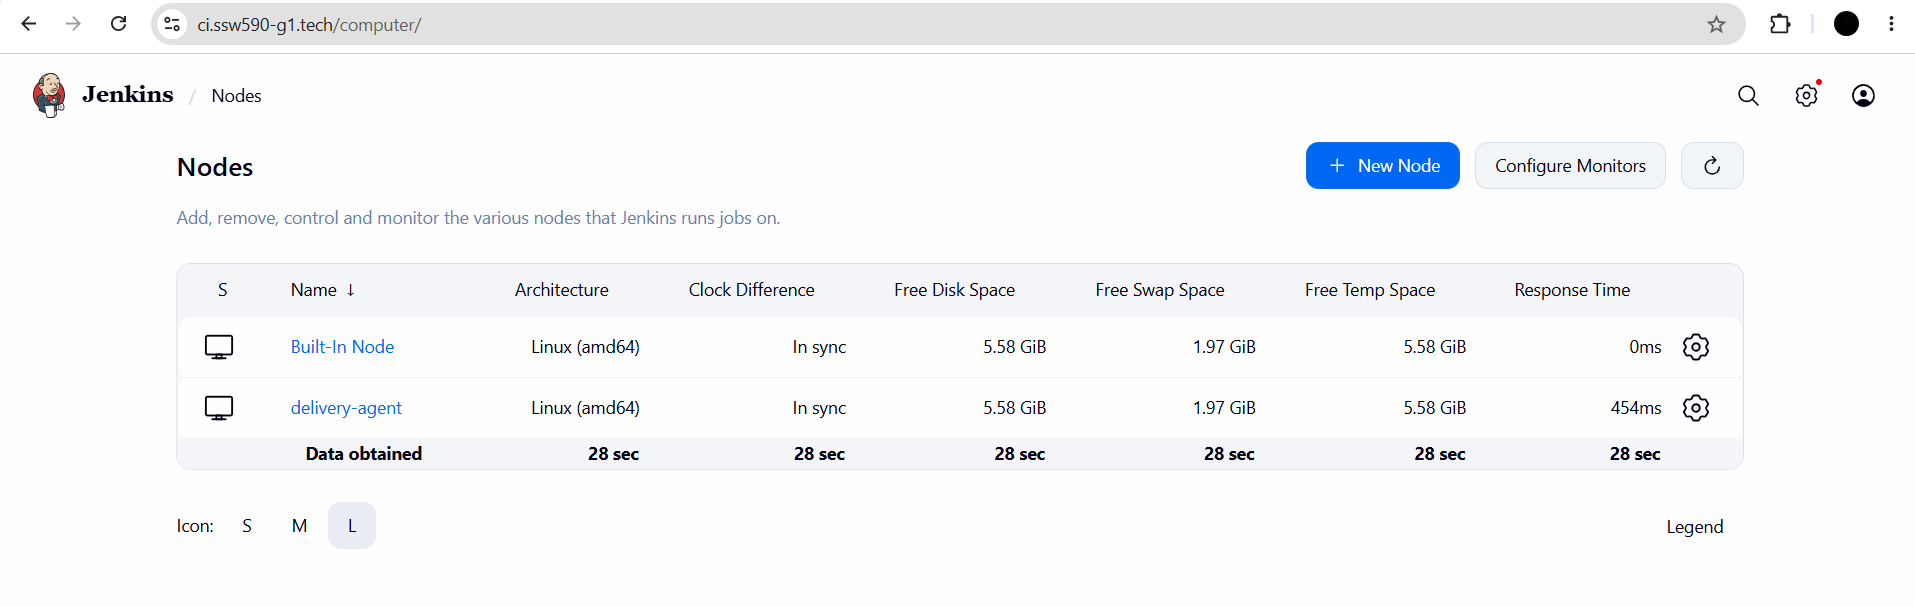
\includegraphics[width=0.9\linewidth]{evidence/206-jenkins-nodes-delivery-agent-linux-online-bd-2026-11-13.png}
\caption{Jenkins Nodes page: \texttt{delivery-agent} online as Linux (BD's screenshot).}
\label{Fig:E206}
\end{figure}

\begin{figure}[htbp]
\centering
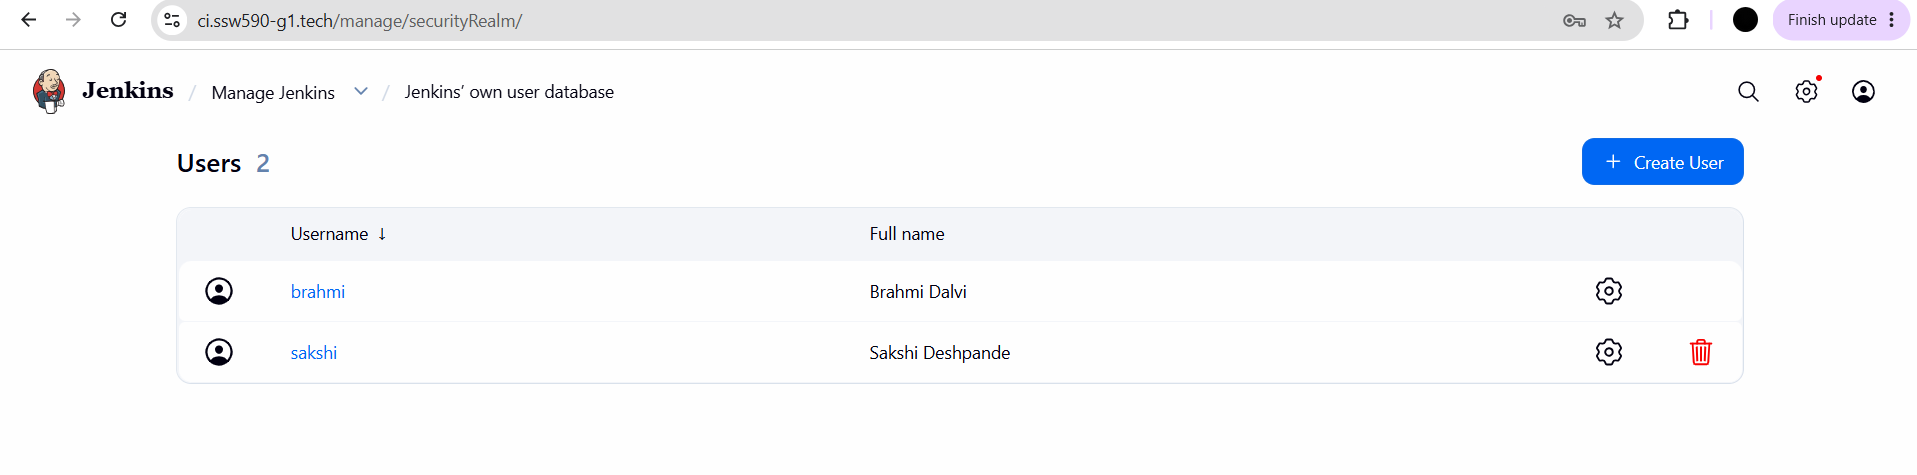
\includegraphics[width=0.9\linewidth]{evidence/210-jenkins-users-brahmi-sakshi-approver-ids-bd-2026-11-14.png}
\caption{The two Jenkins users, \texttt{brahmi} and \texttt{sakshi}, the only approvers (BD's screenshot).}
\label{Fig:E210}
\end{figure}

\begin{longlisting}
\inputminted[fontsize=\scriptsize]{text}{evidence/212-first-delivery-run-build-5-pip-audit-cache-failure-and-fix-bd-2026-11-16.txt}
\caption{Build \#5: the first delivery run failed on a root-owned cache directory, and the fix (real output).}
\label{Listing:E212}
\end{longlisting}

\begin{figure}[htbp]
\centering
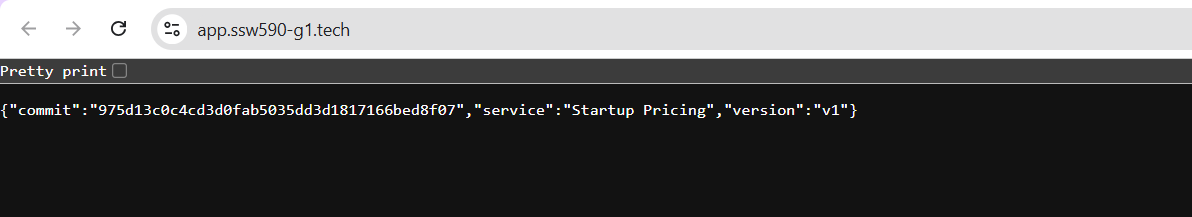
\includegraphics[width=0.9\linewidth]{evidence/218-app-ssw590-g1-tech-v1-in-browser-bd-2026-11-17.png}
\caption{The production URL in a browser after the first release (BD's screenshot).}
\label{Fig:E218}
\end{figure}

\begin{figure}[htbp]
\centering
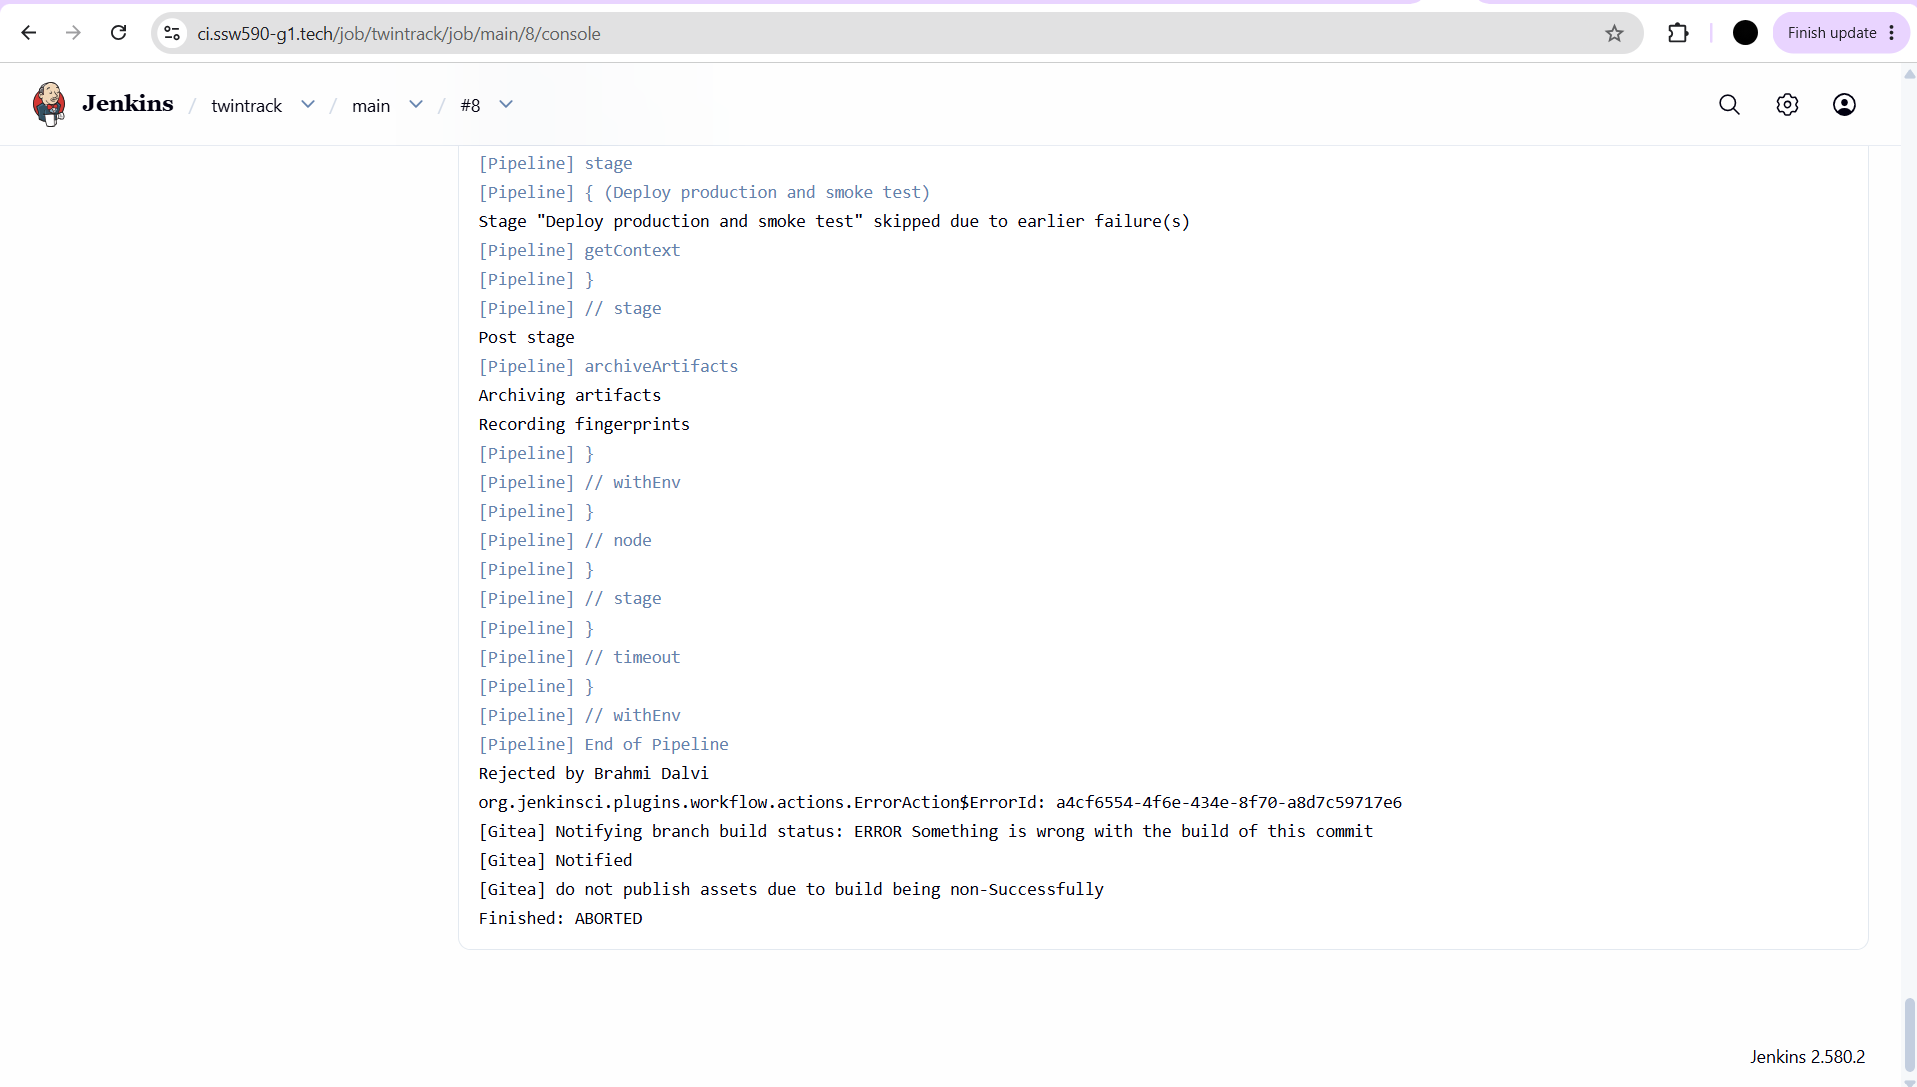
\includegraphics[width=0.9\linewidth]{evidence/221-build-8-aborted-rejected-by-brahmi-bd-2026-11-17.png}
\caption{Build \#8 ends \emph{Rejected by Brahmi Dalvi}: staged, not promoted (BD's screenshot).}
\label{Fig:E221}
\end{figure}

\begin{longlisting}
\inputminted[fontsize=\scriptsize]{text}{evidence/216-build-7-v1-released-staging-then-production-same-digest-bd-2026-11-17.txt}
\caption{Build \#7, November 17, 2026: v1 to staging, approval by \texttt{brahmi}, the same digest to production (real output).}
\label{Listing:E216}
\end{longlisting}

\begin{figure}[htbp]
\centering
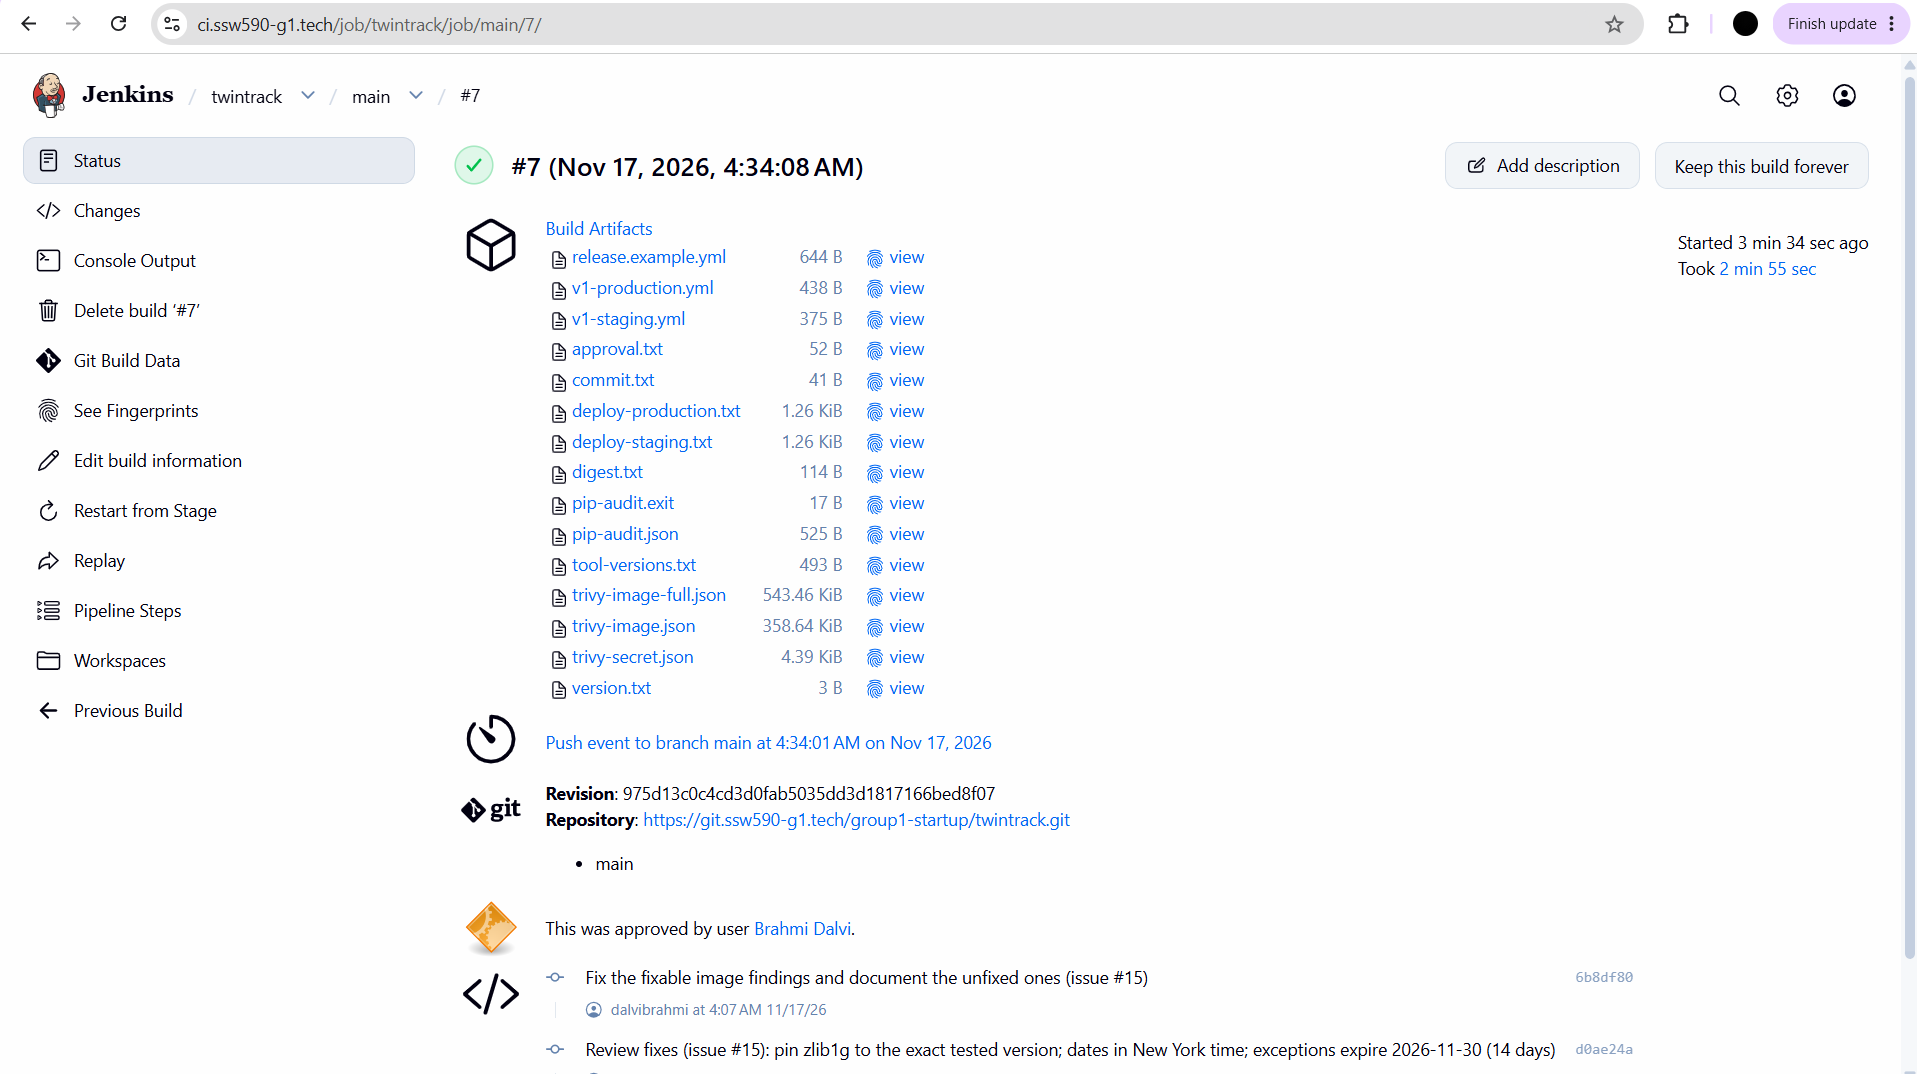
\includegraphics[width=0.9\linewidth]{evidence/217-build-7-success-artifacts-approved-by-brahmi-bd-2026-11-17.png}
\caption{Jenkins build \#7: success, 16 archived artifacts, ``approved by user Brahmi Dalvi'' (BD's screenshot).}
\label{Fig:E217}
\end{figure}

\begin{figure}[htbp]
\centering
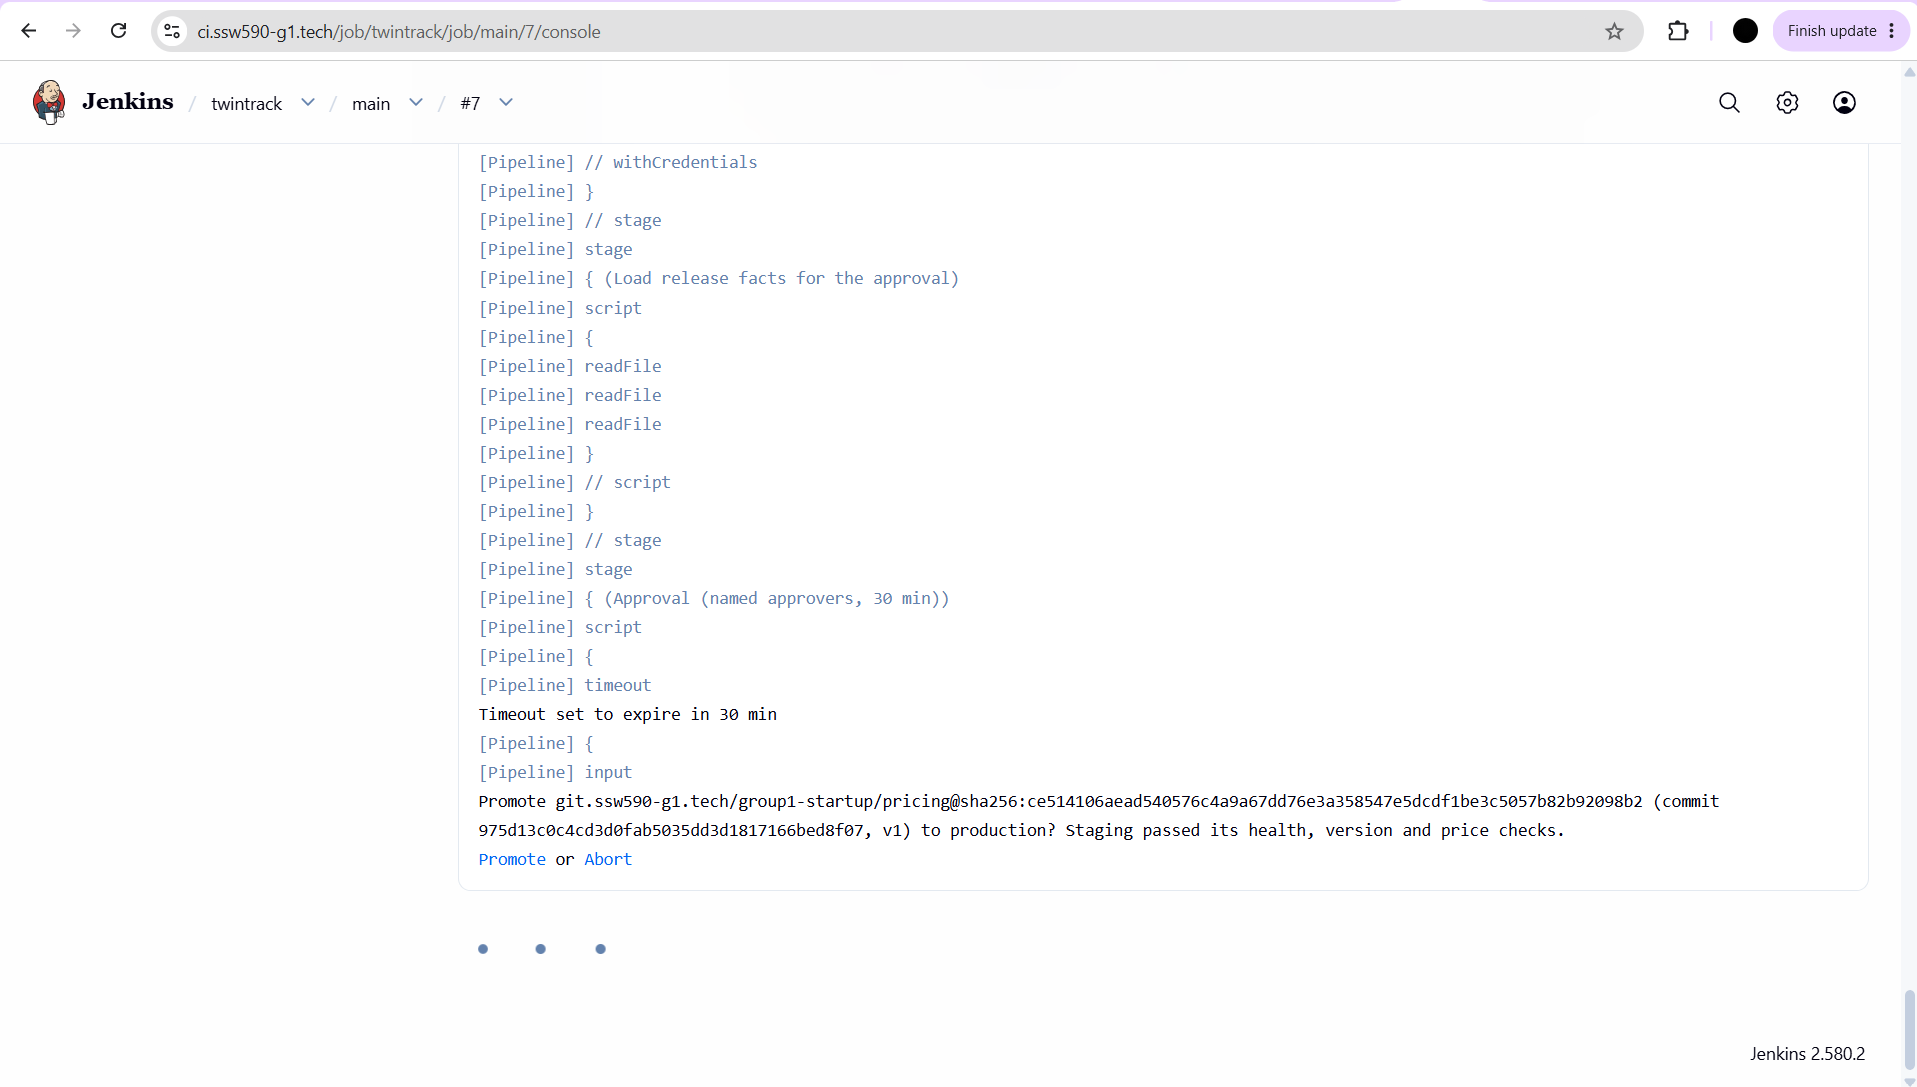
\includegraphics[width=0.9\linewidth]{evidence/214-build-7-approval-prompt-promote-or-abort-bd-2026-11-17.png}
\caption{The approval prompt of build \#7: digest, commit, version, Promote or Abort, 30-minute timeout (BD's screenshot).}
\label{Fig:E214}
\end{figure}

\begin{figure}[htbp]
\centering
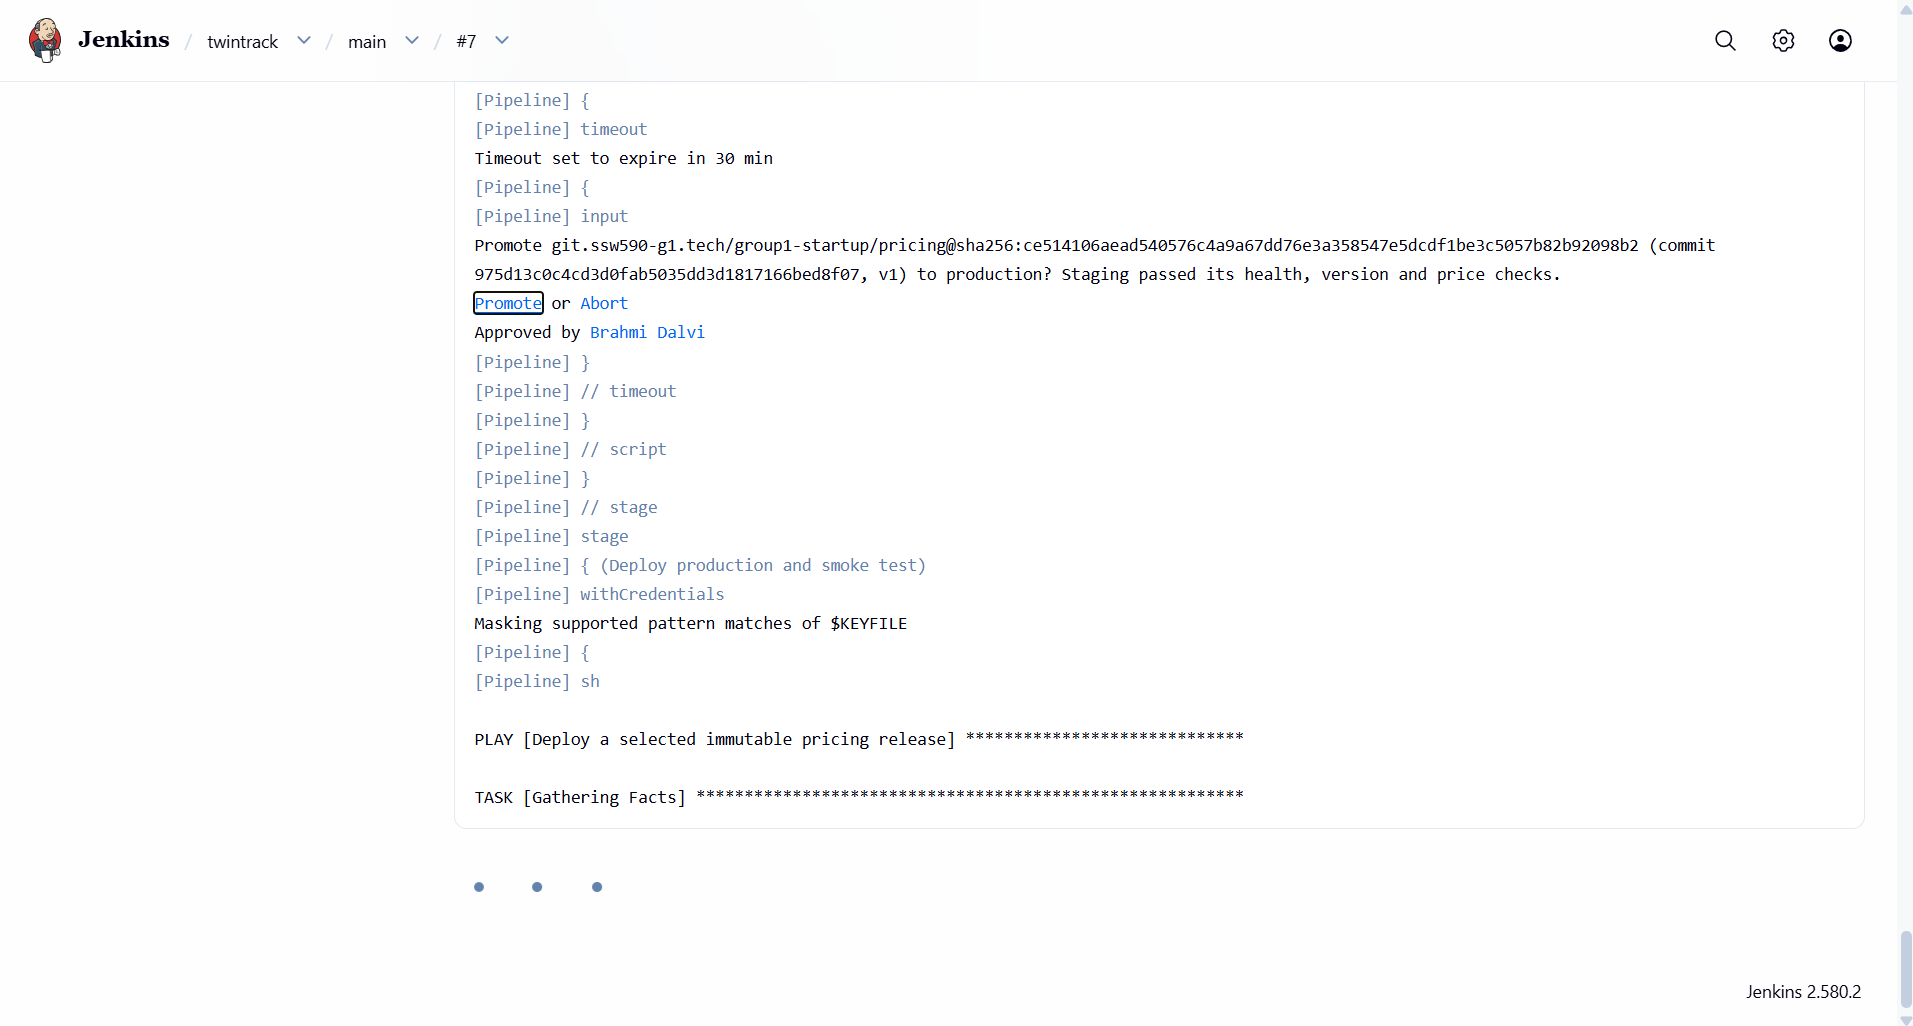
\includegraphics[width=0.9\linewidth]{evidence/215-build-7-approved-by-brahmi-production-deploy-started-bd-2026-11-17.png}
\caption{Build \#7 after the click: ``Approved by Brahmi Dalvi'', then the production deploy starts (BD's screenshot).}
\label{Fig:E215}
\end{figure}

\begin{longlisting}
\inputminted[fontsize=\scriptsize]{text}{evidence/230-build-11-v2-staging-verified-before-promotion-bd-2026-11-18.txt}
\caption{Build \#11 (v2) before promotion: scans, the staging record and public checks (real output).}
\label{Listing:E230}
\end{longlisting}

\begin{figure}[htbp]
\centering
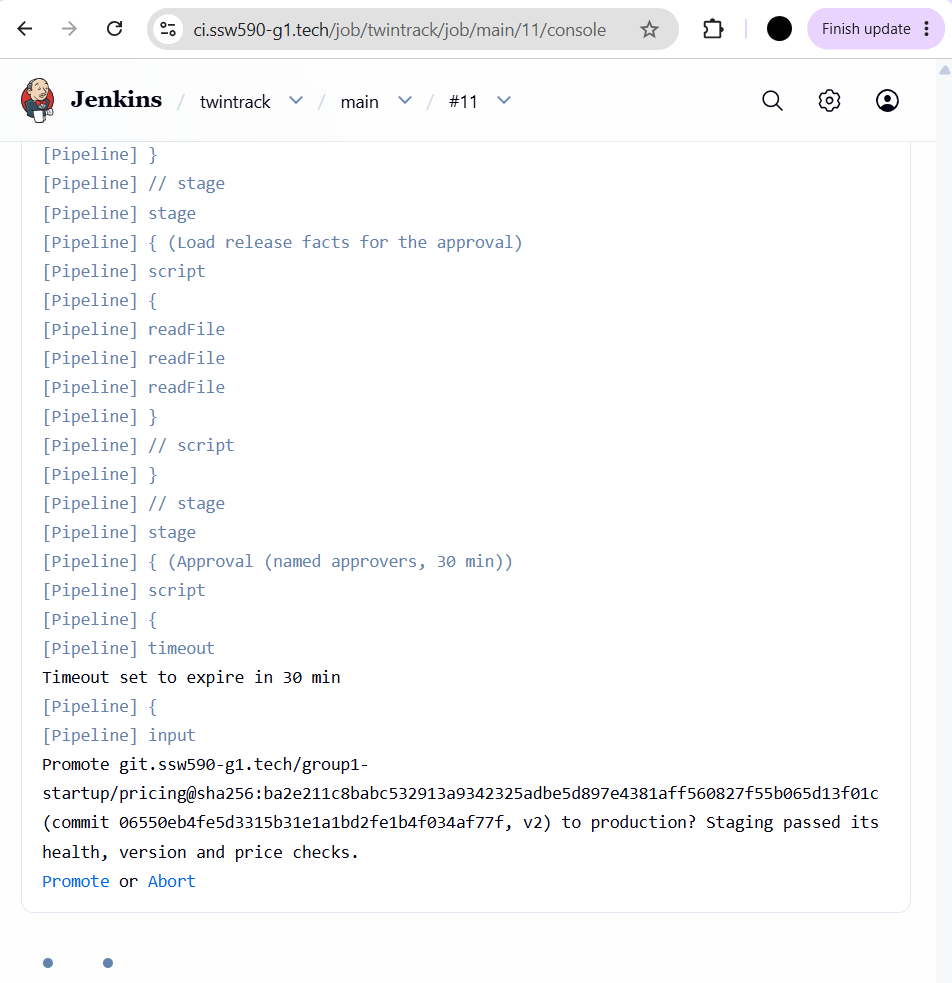
\includegraphics[width=0.9\linewidth]{evidence/229-build-11-v2-approval-prompt-bd-2026-11-18.png}
\caption{The approval prompt of build \#11 (v2) (BD's screenshot).}
\label{Fig:E229}
\end{figure}

\begin{longlisting}
\inputminted[fontsize=\scriptsize]{text}{evidence/231-build-11-v2-promoted-production-serves-v2-total-36-bd-2026-11-18.txt}
\caption{v2 promoted to production, November 17, 2026, 21:21~EST (real output).}
\label{Listing:E231}
\end{longlisting}

\begin{figure}[htbp]
\centering
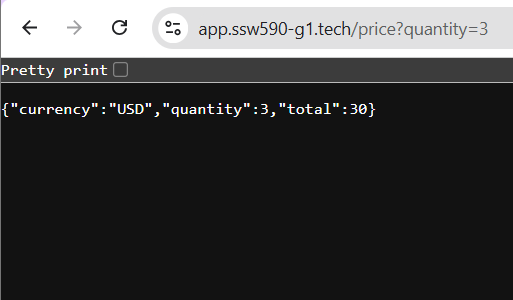
\includegraphics[width=0.9\linewidth]{evidence/235-app-price-quantity-3-total-30-after-rollback-in-browser-bd-2026-11-18.png}
\caption{Production after the v2 release: \texttt{/price?quantity=3} (BD's screenshot taken after the rollback of Section~\ref{Section:deliveryRecovery}).}
\label{Fig:E235}
\end{figure}

\begin{longlisting}
\inputminted[fontsize=\scriptsize]{text}{evidence/222-build-8-merge-of-pr-22-staged-not-promoted-aborted-bd-2026-11-17.txt}
\caption{Build \#8: staged, not promoted, aborted at the approval (real output).}
\label{Listing:E222}
\end{longlisting}

\begin{longlisting}
\inputminted[fontsize=\scriptsize]{text}{evidence/223-build-9-release-records-pr-19-delivery-skipped-by-changeset-bd-2026-11-17.txt}
\caption{Build \#9, the merge of the release-records pull request: the delivery stage is skipped (real output).}
\label{Listing:E223}
\end{longlisting}


% ===== BD region: row 5 (15 points) =====
\section{Security scans, policy and credentials (15 points)}\label{Section:deliveryScans}
\textbf{Owner:} BD. \textbf{Status:} policy written before the first release; one real block and one synthetic block recorded \StatusPass; the instructor's acceptance of the dated exceptions is requested.

\paragraph{Policy (written before the release).} The file \texttt{scan-policy.md} (course repository, \texttt{assignment-8/bd-work}) fixes what is scanned, when, and what blocks:
\begin{tabularx}{\linewidth}{L{3.2cm}L{3.2cm}Y}
\caption{Scan policy\label{Table:ScanPolicy}}\\
\toprule \textbf{What} & \textbf{Tool} & \textbf{When and what blocks}\\ \midrule
\endfirsthead
\toprule \textbf{What} & \textbf{Tool} & \textbf{When and what blocks}\\ \midrule
\endhead \bottomrule \endlastfoot
Python dependencies & pip-audit 2.10.1 on the hashed lock & before the build; any known vulnerability, a scanner error, or a missing report blocks.\\
Secrets in the source & Trivy 0.76.2, file-system secret scan & before the build; any finding blocks.\\
Image & Trivy image scan, HIGH and CRITICAL & after the build, before the push; any finding not covered by a dated exception blocks.\\
\end{tabularx}
Fixes come first. A finding with a fixed version is fixed (bump the dependency or the base, rebuild, rescan). An unfixed finding needs a written exception with the identifier, the reason, an owner and an expiry no later than 14 days,
reviewed in a pull request by the other person; an expired exception blocks again. There is no \texttt{|| true} anywhere in the pipeline.

\paragraph{The gate on the real release.} Build \#6 passed tests, pip-audit and the secret scan, built the image, and then the image scan stopped it: 53 HIGH findings and no CRITICAL, 47 of them without any fixed version (\ListRef{213}).
Nothing was pushed or deployed. Six findings had a fix and were fixed in the Dockerfile in pull request \#16 (the \texttt{zlib1g} security update, pinned to the exact version read from the tested image, and \texttt{pip}, \texttt{setuptools} and \texttt{wheel} removed
after the locked install, which also removed the vendored urllib3, msgpack and setuptools findings). The 47 rows are 11 CVE identifiers in Debian base-image packages (util-linux, acl, ncurses, sqlite, systemd and perl); each is listed in \texttt{.trivyignore.yaml}
with a reason in \texttt{security/exceptions.md}. The base-image findings are about local privilege escalation, mount helpers and libraries the service does not call; the service runs as UID 10001 on a read-only file system with all capabilities dropped.
\textbf{The exceptions expire on 2026-11-30 at 00:00~UTC, that is Sunday, November 29, 2026, 7~pm in New York}; after that every build blocks again until a reviewed pull request renews or removes them. The instructor's acceptance is requested for the use of these exceptions.

\paragraph{What reached the registry.} The package page of the \texttt{pricing} image lists exactly three versions: the commits \texttt{975d13c} (v1, build \#7), \texttt{102da1d} (build \#8, staged and not promoted) and \texttt{06550eb} (v2, build \#11). The image of the blocked build \#6 and nothing of the fixture build \#12 was ever pushed, which is what the order scan, then push, guarantees The page of the v2 version shows the digest the pipeline recorded and the user \texttt{jenkins-bot} as publisher (\FigRef{242}).

\paragraph{After the fix.} Every later build keeps the full report (\texttt{trivy-image-full.json}: 47 HIGH rows) and gates on the filtered one (0 rows). The tested change: the image built from the modified Dockerfile scans with 0 findings and the service
answered \texttt{/health} and \texttt{/price}; the pinned package installed in the real build (\ListRef{213}, \ListRef{216}).

\paragraph{Blocked fixture.} To show each scanner block a bad change without putting anything into the repository, BD replayed build \#11 with a fixture step: a temporary directory with a known-vulnerable pin (urllib3 1.25.8) and a fake credential in the shape of a GitHub token
(assembled at run time, never valid). Result (\ListRef{239}): pip-audit exit 1 with 21 vulnerabilities, Trivy secret scan exit 1 with one CRITICAL finding of rule \texttt{github-pat}, the line \texttt{BLOCKED}, and every later stage (image build, push, staging, approval, production)
skipped; no image was built, nothing was pushed, both environments were untouched, and the temporary directory was removed.

\paragraph{Credentials and access.} Nothing secret is in Git, in the chat with the assistant, in command arguments, or in logs; BD typed or pasted each secret herself.
\begin{tabularx}{\linewidth}{L{3.2cm}L{3.4cm}Y}
\caption{Credentials of the delivery pipeline\label{Table:DeliveryCredentials}}\\
\toprule \textbf{Credential} & \textbf{Where it lives} & \textbf{Scope and risk}\\ \midrule
\endfirsthead
\toprule \textbf{Credential} & \textbf{Where it lives} & \textbf{Scope and risk}\\ \midrule
\endhead \bottomrule \endlastfoot
\texttt{deploy-ssh-key} & Jenkins credential only (\FigRef{204}); the local key files were deleted & ed25519 key for the \texttt{deploy} account: key-only login, no password, passwordless \texttt{sudo} (documented as host-administrator power, \ListRef{203}); revoke by deleting the line in \texttt{authorized\_keys}.\\
\texttt{gitea-registry-write} & Jenkins credential, bound only in the push stage & Gitea user \texttt{jenkins-bot}, package scope only, with an expiry (\FigRef{207}); the account has more rights in the \texttt{developers} team (\FigRef{209}), so the token is narrower than the account.\\
registry read token & root's \texttt{/root/.docker/config.json} on the host & read-only, with an expiry; stored in plain text, readable by root and so by the \texttt{deploy} account and the agent; used for the pull by digest (\ListRef{211}).\\
Jenkins users & Jenkins' own database & exactly \texttt{brahmi} and \texttt{sakshi} may approve (\FigRef{210}).\\
\end{tabularx}
The deploy path is the host's Docker bridge (alias \texttt{deploy-target}) with a pinned SSH host key, because the host cannot reach its own Elastic IP on port 22 through the security group (\ListRef{201}). The two public hostnames, \texttt{staging} and \texttt{app}, are served by Caddy with
Let's Encrypt certificates issued within seconds of the reload (\ListRef{208}); both are public on purpose because the service is stateless and Ansible checks the public name.

\begin{longlisting}
\inputminted[fontsize=\scriptsize]{text}{evidence/213-build-6-image-scan-gate-blocked-the-release-bd-2026-11-16.txt}
\caption{Build \#6, November 16, 2026: the image scan blocked the release (real output).}
\label{Listing:E213}
\end{longlisting}

\begin{longlisting}
\inputminted[fontsize=\scriptsize]{text}{evidence/239-blocked-fixture-secret-and-vulnerable-dependency-bd-2026-11-18.txt}
\caption{Blocked fixture: pip-audit and the secret scan stop a replayed build (real output).}
\label{Listing:E239}
\end{longlisting}

\begin{longlisting}
\inputminted[fontsize=\scriptsize]{text}{evidence/201-ssh-reachability-from-host-and-containers-to-own-public-and-private-address-bd-2026-11-12.txt}
\caption{SSH from the host and from containers to its own public and private address (real output).}
\label{Listing:E201}
\end{longlisting}

\begin{longlisting}
\inputminted[fontsize=\scriptsize]{text}{evidence/208-caddy-blocks-staging-and-app-applied-certificates-issued-bd-2026-11-14.txt}
\caption{The two Caddy blocks for staging and app; the certificates are issued (real output).}
\label{Listing:E208}
\end{longlisting}

\begin{longlisting}
\inputminted[fontsize=\scriptsize]{text}{evidence/203-deploy-account-created-key-only-sudo-bd-2026-11-12.txt}
\caption{The deploy account (real output pasted by BD).}
\label{Listing:E203}
\end{longlisting}

\begin{figure}[htbp]
\centering
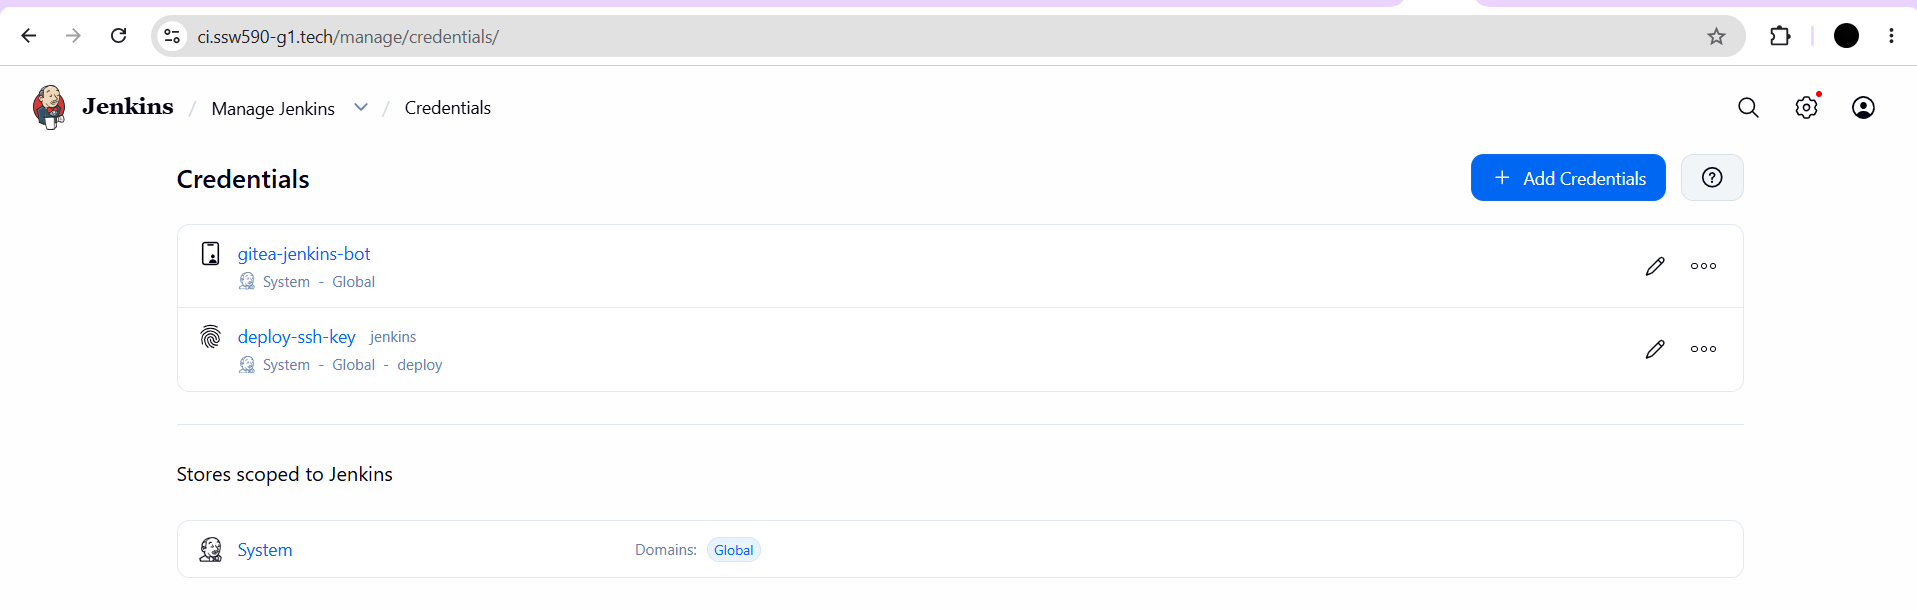
\includegraphics[width=0.9\linewidth]{evidence/204-jenkins-credentials-list-deploy-ssh-key-added-bd-2026-11-12.png}
\caption{Jenkins credentials after the deploy key was added (BD's screenshot).}
\label{Fig:E204}
\end{figure}

\begin{figure}[htbp]
\centering
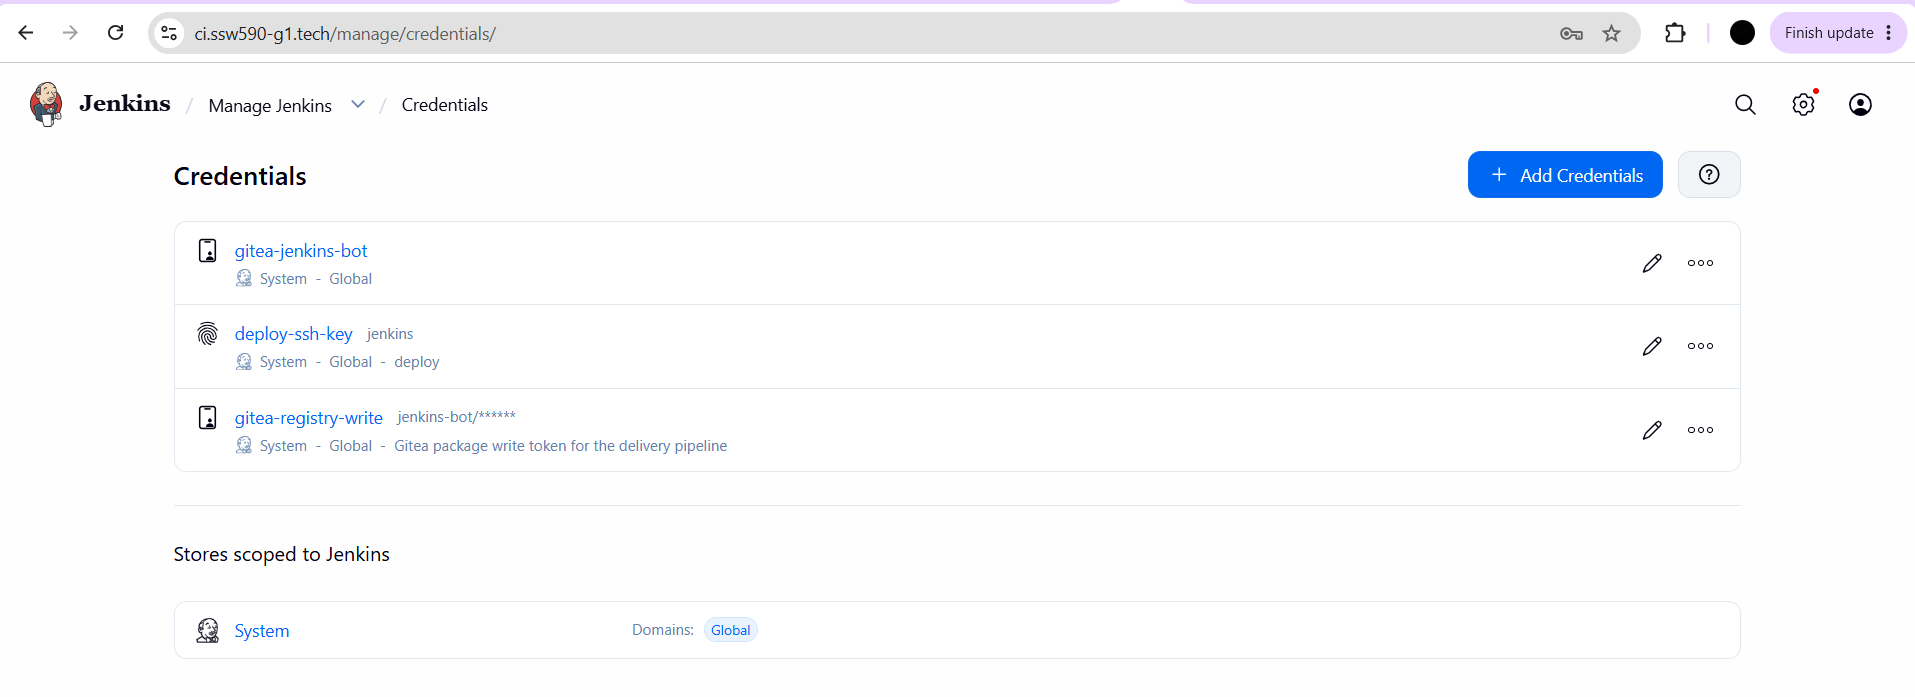
\includegraphics[width=0.9\linewidth]{evidence/207-jenkins-credentials-gitea-registry-write-added-bd-2026-11-14.png}
\caption{Jenkins credentials after the registry write credential was added; the token is masked (BD's screenshot).}
\label{Fig:E207}
\end{figure}

\begin{figure}[htbp]
\centering
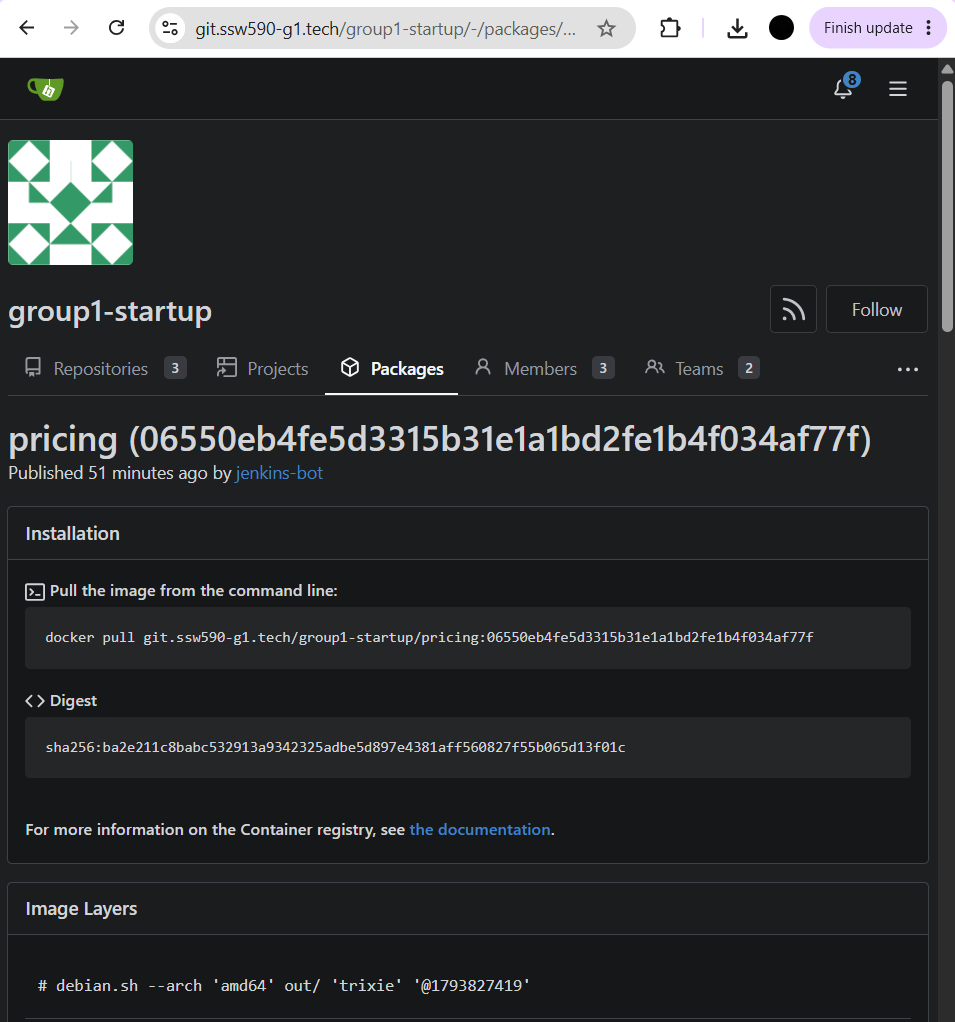
\includegraphics[width=0.9\linewidth]{evidence/242-gitea-package-pricing-v2-published-by-jenkins-bot-digest-bd-2026-11-18.png}
\caption{The package page of the v2 image: published by \texttt{jenkins-bot}, digest \texttt{sha256:ba2e211c\ldots f01c} (BD's screenshot).}
\label{Fig:E242}
\end{figure}

\begin{figure}[htbp]
\centering
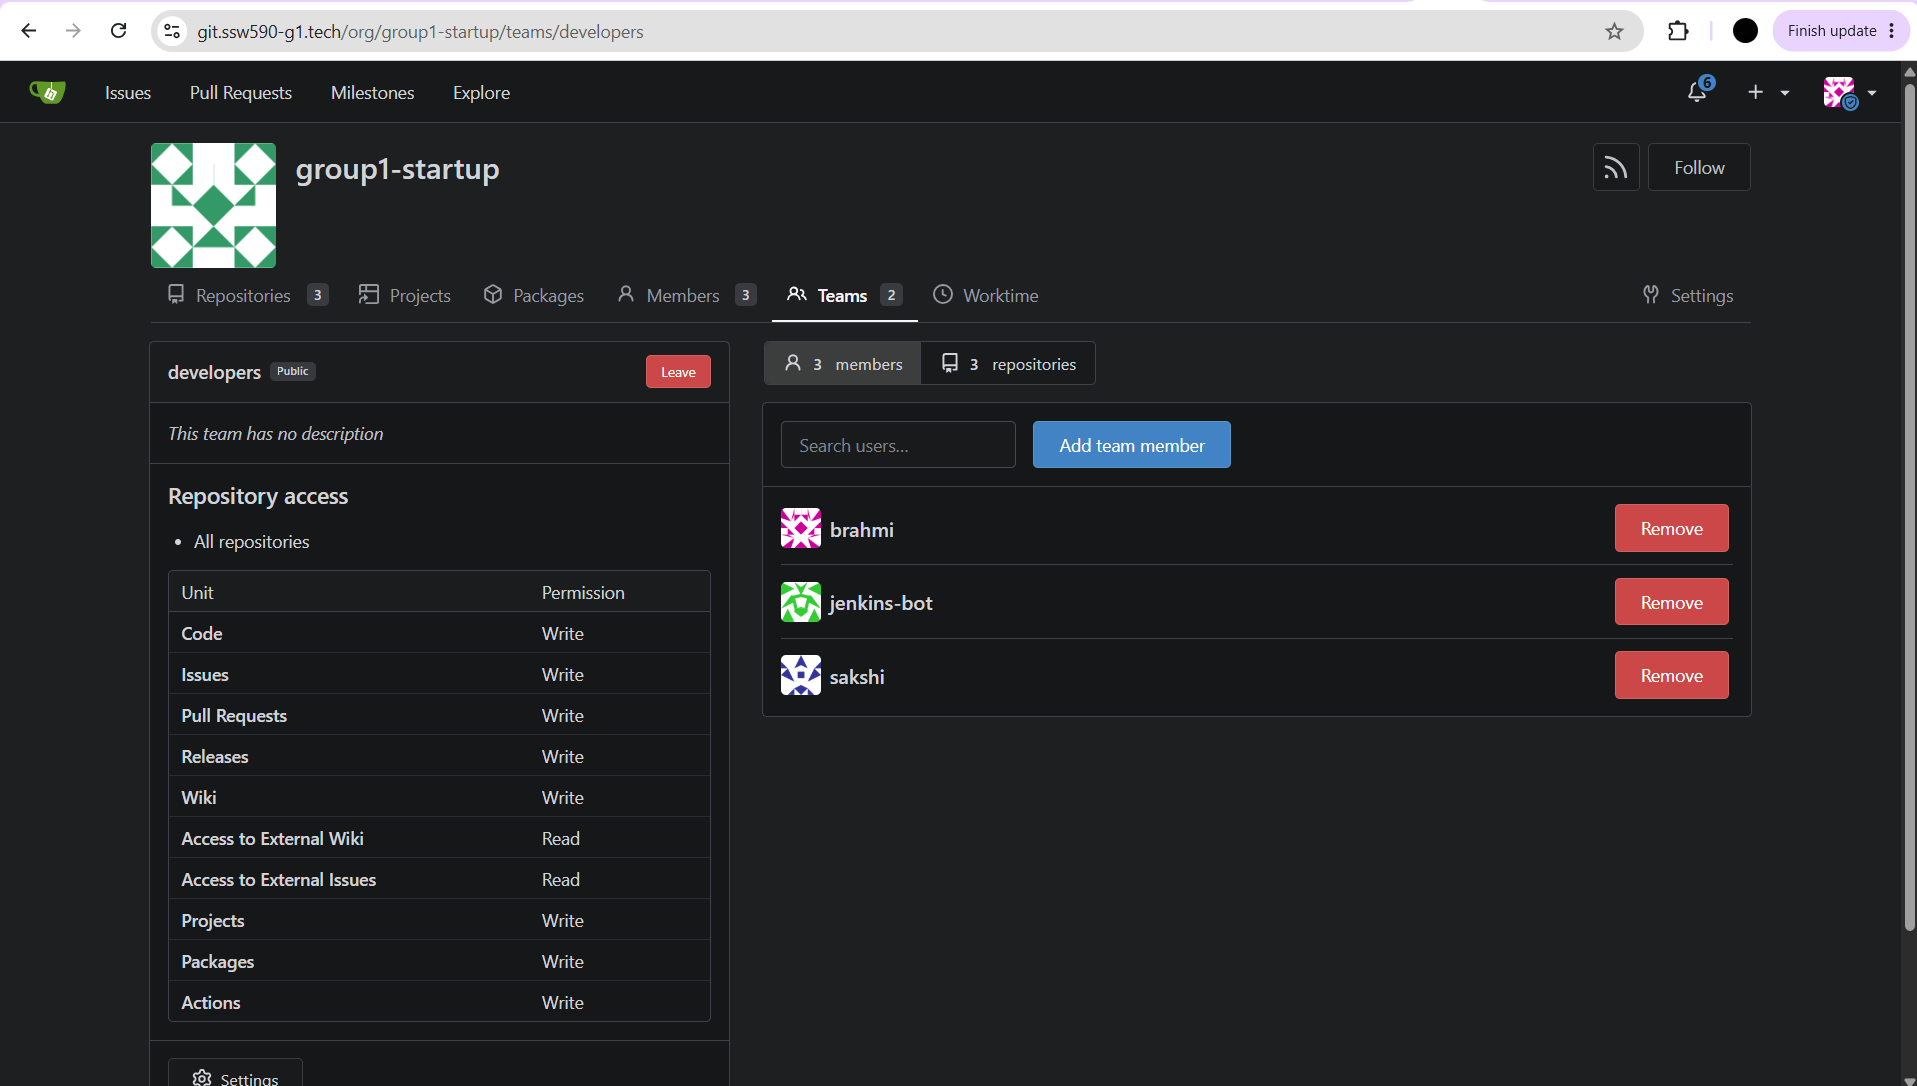
\includegraphics[width=0.9\linewidth]{evidence/209-gitea-developers-team-jenkins-bot-packages-write-bd-2026-11-14.png}
\caption{The \texttt{developers} team: \texttt{jenkins-bot} has Packages write (BD's screenshot).}
\label{Fig:E209}
\end{figure}

\begin{longlisting}
\inputminted[fontsize=\scriptsize]{text}{evidence/211-registry-read-login-root-and-pre-merge-check-bd-2026-11-16.txt}
\caption{Root's registry login and the pre-merge check (real output pasted by BD).}
\label{Listing:E211}
\end{longlisting}


% ===== BD region: row 6 (15 points) =====
\section{Rollback and staging recovery (15 points)}\label{Section:deliveryRecovery}
\textbf{Owner:} BD. \textbf{Status:} both recoveries run on November 17, 2026 (New York) \StatusPass.

\paragraph{The mechanism.} Both recoveries re-apply a \emph{release record} (exact digest, commit, expected version and total, public URL, network) with the same Ansible playbook as a normal release; nothing is rebuilt and no tag such as \texttt{latest} is used.
A second Jenkins job, \texttt{rollback} (file \texttt{Jenkinsfile.rollback}), accepts only \texttt{releases/v<n>-staging.yml} or \texttt{-production.yml}, checks that the record is tracked in \texttt{main}, that its \texttt{target\_env} agrees with the name, that the image is a digest, that the commit is 40 hexadecimal
characters and an ancestor of \texttt{main}, so a rollback cannot target an unreviewed release; a production record needs the same named approval, a staging record does not.
The v1 records are committed in \texttt{main} (pull request \#19, byte-identical to the archived artifacts of build \#7).

\paragraph{Three problems before it ran.} Builds \#1 to \#4 of the job failed without touching any server: the file was not on \texttt{main} yet; then Jenkins refused the whole file because of an invalid Groovy escape (a backslash-dot in a regular expression inside a triple-quoted
shell block): ``unexpected char: \textbackslash{}'' (\FigRef{224}, \ListRef{225}). BD's local checks missed it because they tested the unescaped shell text; a check script that finds invalid escapes was added, and the fix went through its own pull request (\#24). The first run of the fixed file stopped
at an unset parameter, which is the safe behaviour of \texttt{set -u}, and registered the parameter.

\paragraph{Unchanged second run (row 3).} With \texttt{releases/v1-staging.yml}: the first run changed 2 tasks (staging moved back from a staged candidate to the build \#7 digest), the second run of the same record showed \texttt{changed=0} and the container was not restarted; the production record, approved by BD, also showed \texttt{changed=0}
(\ListRef{228}).

\paragraph{Case A: production rollback v2 to v1 (job \texttt{rollback}, build \#8).} Trigger: v2 live in production. BD chose the record \texttt{releases/v1-production.yml}; the prompt named the digest \texttt{sha256:ce514106\ldots 98b2} (\FigRef{226}); BD approved at 02:23:37~UTC on November 18 (\FigRef{227});
Ansible ended \texttt{ok=9 changed=2 failed=0} and its smoke test asserted version v1, the right commit and total 30. The container started 12~seconds after the approval; public checks: version v1, commit \texttt{975d13c}, total 30 (\FigRef{234}, \FigRef{235}, \ListRef{232}).
A read-only observer on the server asked the production URL once a second (\ListRef{233}): the last v2 answer at 02:23:48, one 502 sample at 02:23:50, the first v1 answer at 02:23:51, that is about 2 to 3~seconds without a good answer, and the only non-200 line. The matching configuration came back with it: the rendered Compose file names the v1 digest again.

\paragraph{Case B: staging failed deployment and recovery.} The failure was injected on purpose and traceably by replaying rollback build \#6 (the replay is build \#9 of the job) with the digest replaced by 64 zeros, an image that does not exist (the deploy key lives only in Jenkins and the job refuses records that are not in \texttt{main}, so a replay is the safe way).
Ansible failed at \emph{Converge application without rebuilding} with ``manifest unknown'', recap \texttt{ok=4 changed=1 failed=1} (\ListRef{237}). Compose pulls the image before it touches the running container, so staging stayed on the v2 container, healthy, still answering v2 and 36; only the rendered Compose file had changed to name the missing digest, a drift between configuration and running release.
Production was untouched and the approval and production stages are never reached after a failed staging deploy. Recovery: the same job as a normal run (build \#10) with \texttt{releases/v1-staging.yml}, \texttt{ok=9 changed=2 failed=0} (the Compose file restored, staging moved onto the known-good digest), verified at 02:46~UTC: version v1, commit \texttt{975d13c}, total 30 on both URLs (\ListRef{238}).
About 6~minutes passed between the failure and the verified recovery, most of it waiting for the person to start the second run. Staging ends on v1, the last release whose record is in \texttt{main}; to put v2 back, its record is committed in a reviewed pull request first.

\paragraph{What is not claimed.} The rollback was practised on a release whose previous version is still in the registry; if a registry image were deleted, a rollback to it would fail like Case B. The runs were short because the service is a single stateless container; a service with data would need a data plan that this exercise does not cover.

\begin{longlisting}
\inputminted[fontsize=\scriptsize]{text}{evidence/228-restore-runs-staging-twice-and-production-changed-0-bd-2026-11-18.txt}
\caption{The three restore runs: staging record twice, then the production record (real output).}
\label{Listing:E228}
\end{longlisting}

\begin{figure}[htbp]
\centering
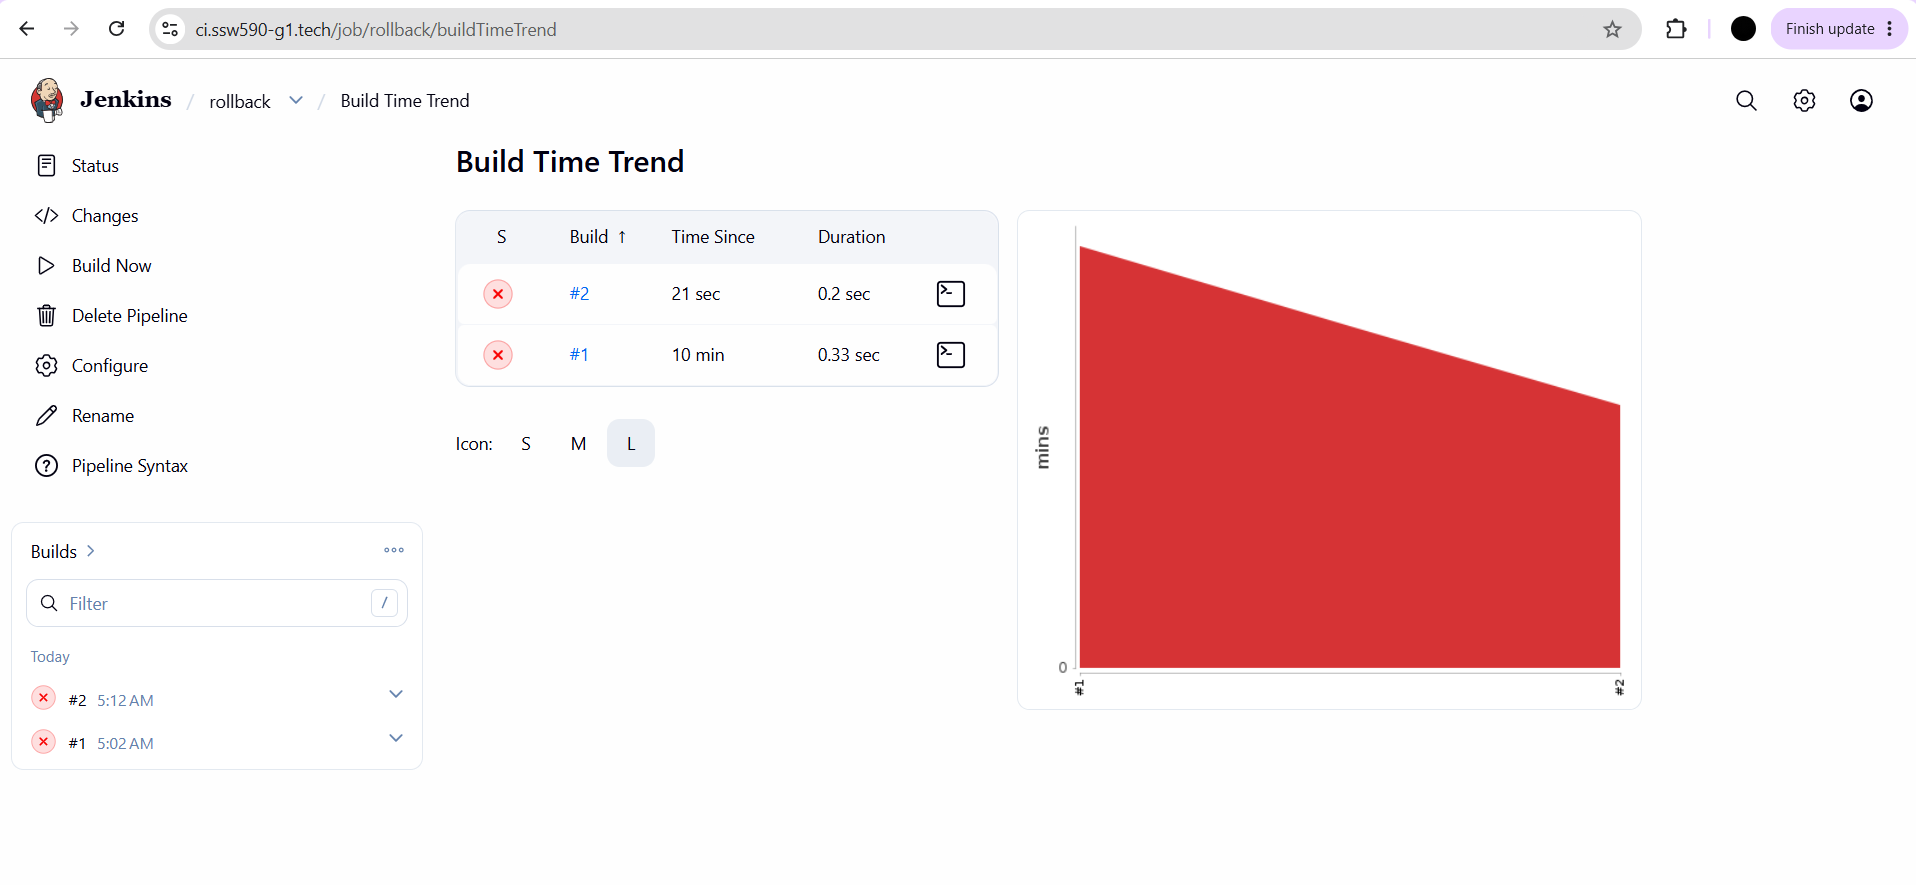
\includegraphics[width=0.9\linewidth]{evidence/224-rollback-job-builds-1-2-failed-groovy-escape-bd-2026-11-17.png}
\caption{The \texttt{rollback} job's first builds failed in under a second (BD's screenshot).}
\label{Fig:E224}
\end{figure}

\begin{longlisting}
\inputminted[fontsize=\scriptsize]{text}{evidence/225-rollback-job-first-runs-failed-groovy-escape-found-and-fixed-bd-2026-11-17.txt}
\caption{Why the first builds failed: an invalid Groovy escape, and the new check (real output).}
\label{Listing:E225}
\end{longlisting}

\begin{figure}[htbp]
\centering
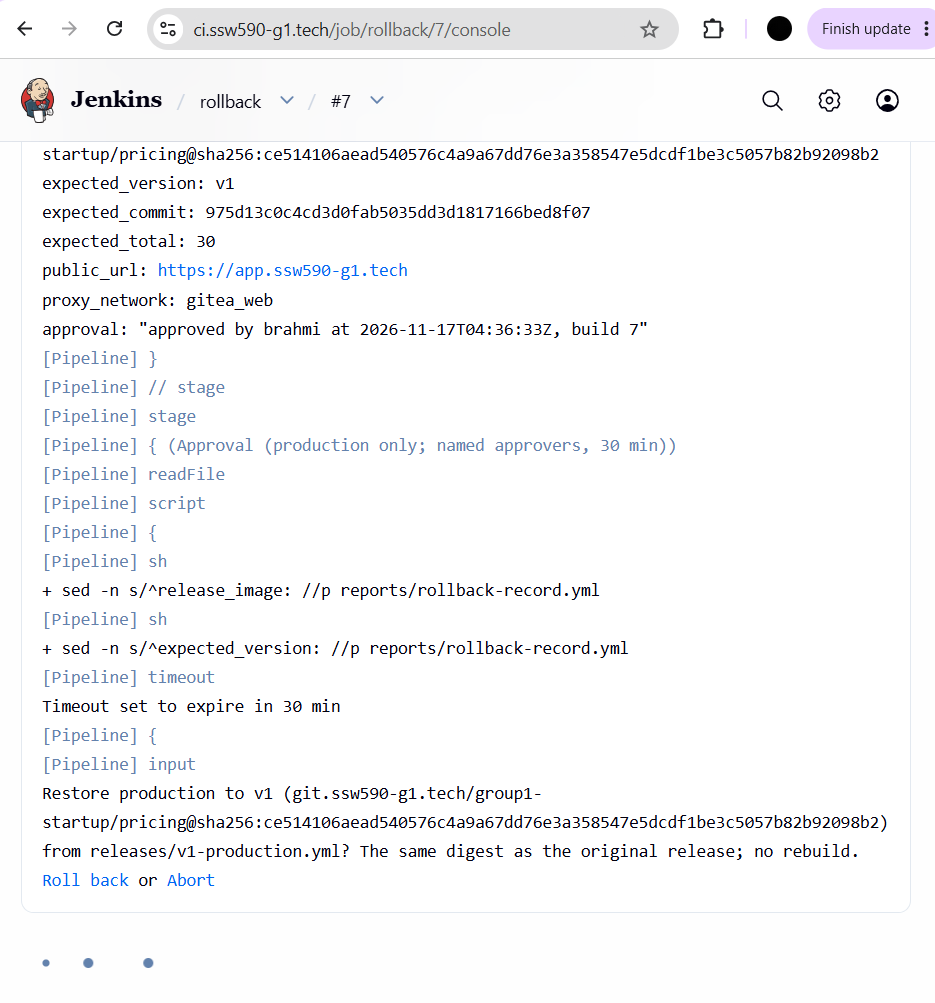
\includegraphics[width=0.9\linewidth]{evidence/226-rollback-job-build-7-approval-prompt-restore-production-v1-bd-2026-11-18.png}
\caption{The approval of the production rollback: the digest of v1, no rebuild (BD's screenshot).}
\label{Fig:E226}
\end{figure}

\begin{figure}[htbp]
\centering
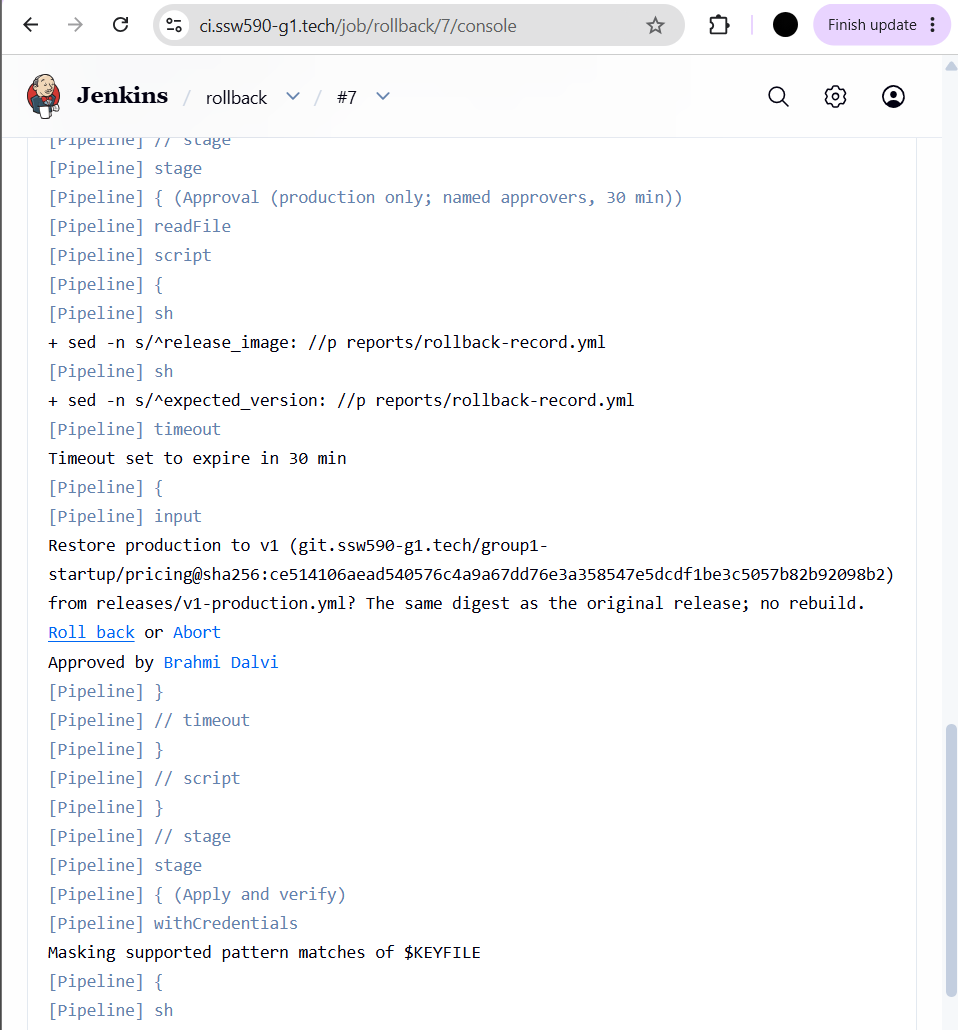
\includegraphics[width=0.9\linewidth]{evidence/227-rollback-job-build-7-approved-by-brahmi-apply-started-bd-2026-11-18.png}
\caption{After the click: ``Approved by Brahmi Dalvi'', Apply and verify starts (BD's screenshot).}
\label{Fig:E227}
\end{figure}

\begin{longlisting}
\inputminted[fontsize=\scriptsize]{text}{evidence/232-production-rollback-v2-to-v1-job-rollback-build-8-bd-2026-11-18.txt}
\caption{The production rollback v2 to v1: record, approval, Ansible, public checks (real output).}
\label{Listing:E232}
\end{longlisting}

\begin{longlisting}
\inputminted[fontsize=\scriptsize,firstline=50,lastline=62]{text}{evidence/233-rollback-observer-log-app-url-per-second-bd-2026-11-18.txt}
\caption{Excerpt of the observer log around the rollback: one request per second to the production URL.}
\label{Listing:E233}
\end{longlisting}

\begin{figure}[htbp]
\centering
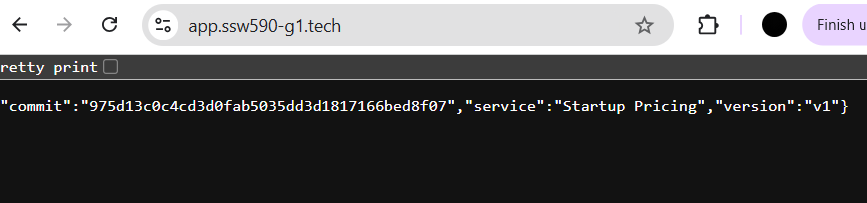
\includegraphics[width=0.9\linewidth]{evidence/234-app-root-v1-after-rollback-in-browser-bd-2026-11-18.png}
\caption{The production URL after the rollback: version v1, commit \texttt{975d13c} (BD's screenshot).}
\label{Fig:E234}
\end{figure}

\begin{longlisting}
\inputminted[fontsize=\scriptsize]{text}{evidence/237-staging-failed-deploy-injected-with-replay-manifest-unknown-bd-2026-11-18.txt}
\caption{The deliberately failed staging deployment: manifest unknown, the running container kept (real output).}
\label{Listing:E237}
\end{longlisting}

\begin{longlisting}
\inputminted[fontsize=\scriptsize]{text}{evidence/238-staging-recovered-to-v1-after-failed-deploy-bd-2026-11-18.txt}
\caption{Staging recovered to v1; the Compose file restored; times (real output).}
\label{Listing:E238}
\end{longlisting}


% ===== BD region: row 7 (5 points) =====
\section{Monitoring correlation and limits (5 points)}\label{Section:deliveryMonitoring}
\textbf{Owner:} BD. \textbf{Status:} production probe added and compared with the releases on November 17, 2026 \StatusPass; no alert reached Discord (reported by BD).

\paragraph{What was added.} The Chapter~\ref{Chapter:Sre} probe job \texttt{https} (Blackbox Exporter, module \texttt{http\_2xx}, 30~second interval) got one more target, the production health URL \texttt{https://app.ssw590-g1.tech/health}.
BD edited the live file herself: the first manual edit was rejected by \texttt{promtool} (a misplaced line and a lost indentation) and was not applied; the second, a one-line \texttt{sed} insert, passed, and Prometheus was restarted
(a single-file bind mount is not re-read on reload); \texttt{probe\_success} was 1 for all three targets (\ListRef{219}, \FigRef{220}). The existing alert rule \texttt{https-service-down} covers every target of the job, so no new rule was needed.
Staging is deliberately \emph{not} probed, so that the planned failed-deploy exercise does not trip the alert. The infrastructure repository copy of the file, together with the Jenkins controller tag and the two Caddy blocks of this assignment, was brought up to date in \texttt{infra} pull request \#8 (issue \#7), merged by BD on November 17, 2026 as merge commit \texttt{a841904}; the change only records what is already live on the server, the \texttt{infra} repository has no written review rule (the contributing rules of \texttt{CONTRIBUTING.md} belong to \texttt{twintrack}), and no review was requested (\FigRef{241}).

\paragraph{What the monitoring showed and what it did not.} Across the v2 promotion at 21:21:44~EST and the rollback at 21:23:37~EST the probe stayed at 1 (\FigRef{236}); the minimum of \texttt{probe\_success} over the previous 10 and 15 minutes was 1 when queried (\ListRef{232}).
The observer on the server saw 2 to 3 seconds without a good answer at the rollback (\ListRef{233}); the probe, with a 30~second scrape interval, never sampled it, and the alert rule, with a 1-minute pending period, cannot fire for a gap that short; BD checked the Discord alerts channel after the runs of the evening of November 17, 2026 and reported that no alert had fired (no screenshot was taken). The same blind spot holds for the 14-second restart of Jenkins (\ListRef{202}).

\paragraph{Limits.} (1) The probe answers 200 for v1 and v2: it shows availability, not whether the price is right; the Ansible smoke test, which checks version, commit and total, is the check that catches a wrong release. (2) A short rollback can fit between two scrapes and be invisible in the metrics. (3) Staging is not probed.
(4) Monitoring runs on the host it watches, so a host outage silences both. (5) The disk is the tight resource (3.5~GB free, 83\% used): the node dashboard and the existing disk alert are the monitoring for it. (6) A release does not yet leave a mark on the dashboard; the correlation is done by hand from the Jenkins times (UTC) and the Prometheus samples.

\begin{longlisting}
\inputminted[fontsize=\scriptsize]{text}{evidence/219-prometheus-probe-for-production-app-added-bd-2026-11-17.txt}
\caption{The production URL added to the probe job (real output pasted by BD).}
\label{Listing:E219}
\end{longlisting}

\begin{figure}[htbp]
\centering
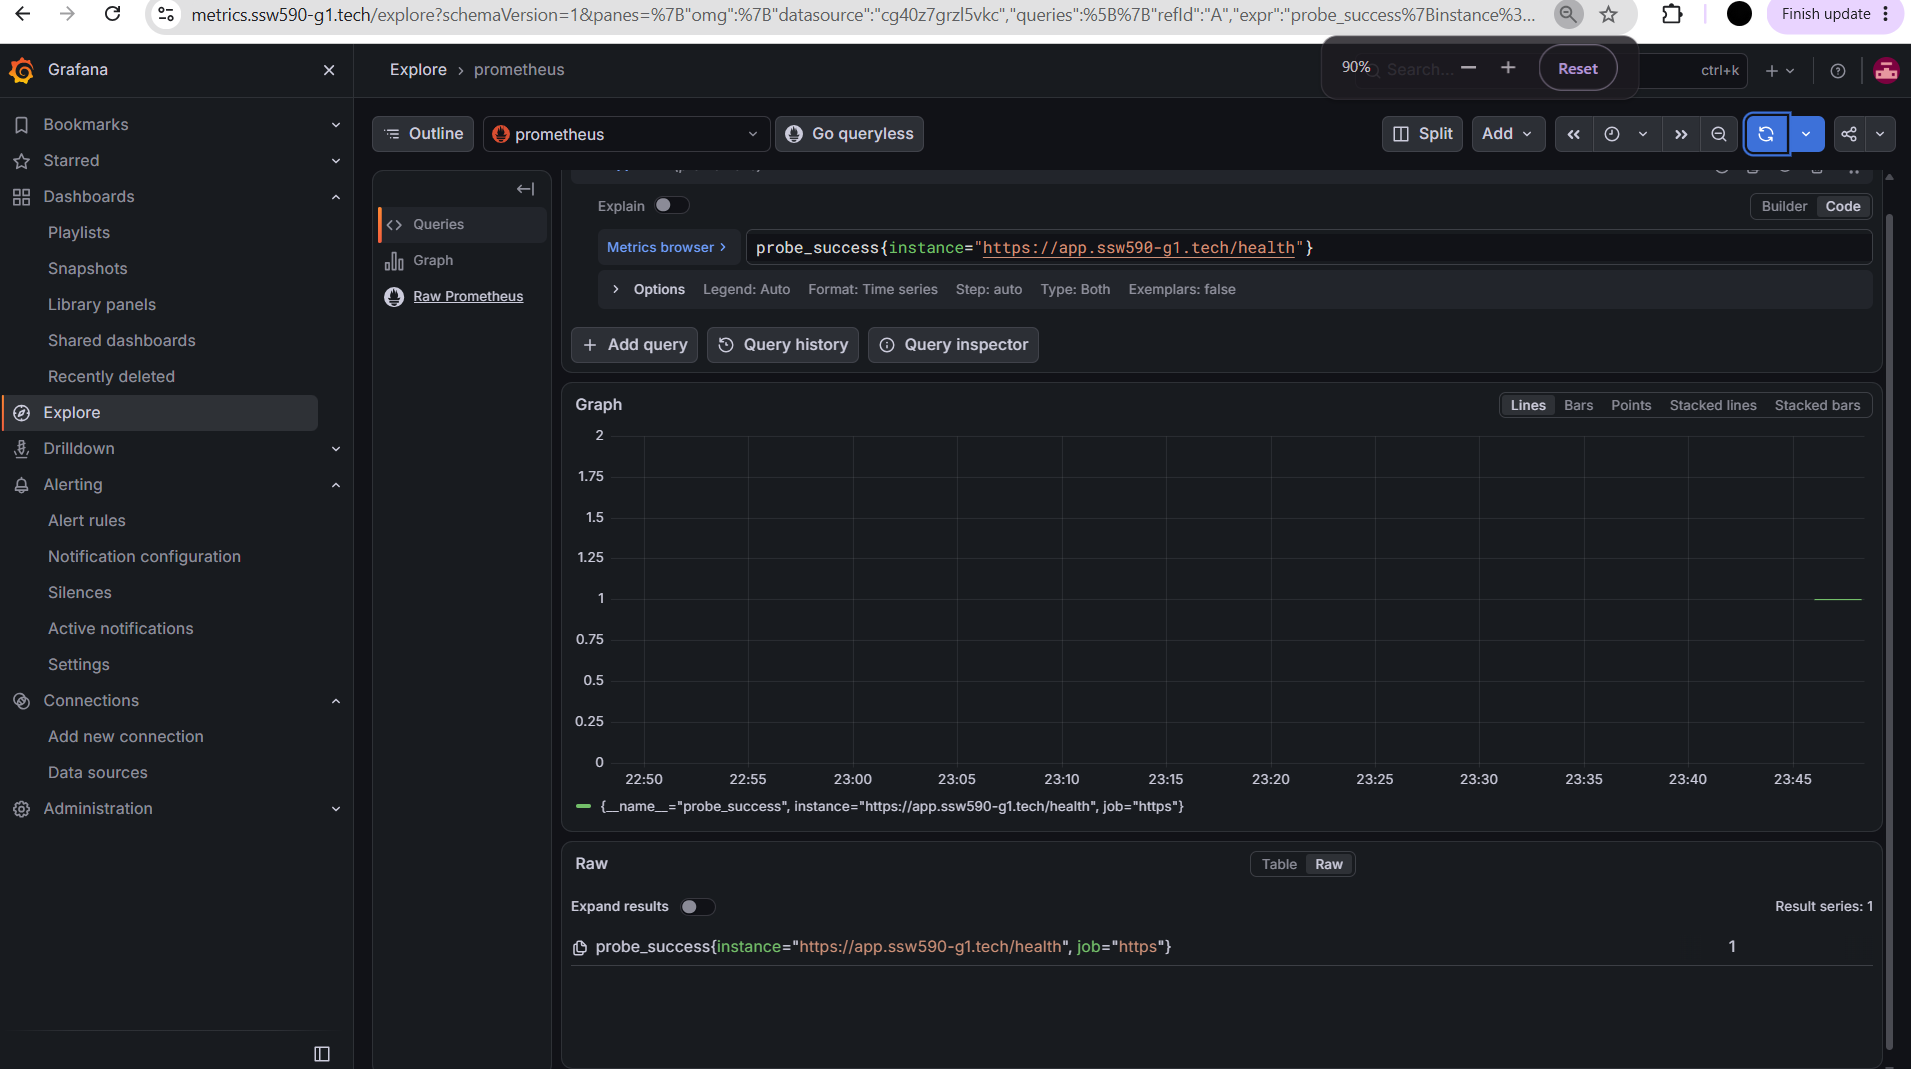
\includegraphics[width=0.9\linewidth]{evidence/220-grafana-explore-probe-success-app-health-bd-2026-11-17.png}
\caption{Grafana Explore: \texttt{probe\_success} of the production URL (BD's screenshot).}
\label{Fig:E220}
\end{figure}

\begin{figure}[htbp]
\centering
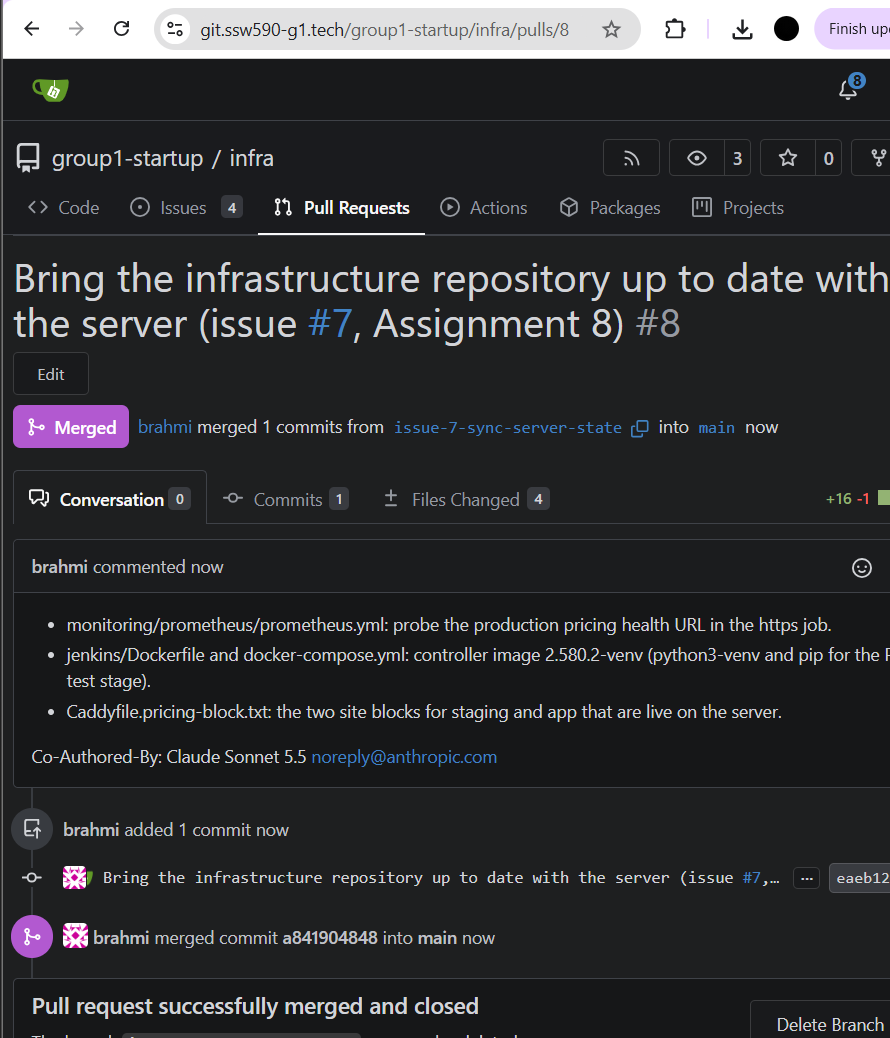
\includegraphics[width=0.9\linewidth]{evidence/241-infra-pr-8-merged-sync-with-server-bd-2026-11-18.png}
\caption{Pull request \#8 of the \texttt{infra} repository, merged: the repository matches the server again (BD's screenshot).}
\label{Fig:E241}
\end{figure}

\begin{figure}[htbp]
\centering
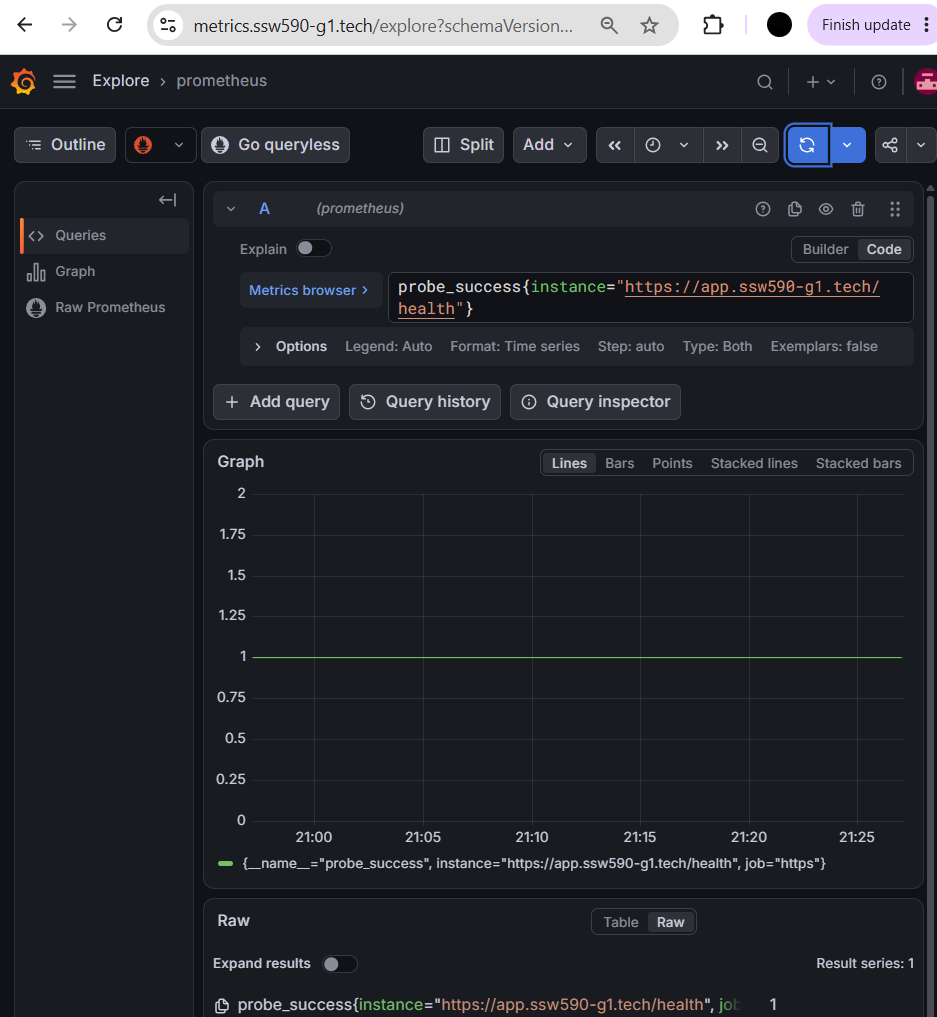
\includegraphics[width=0.9\linewidth]{evidence/236-grafana-explore-probe-success-app-flat-1-through-rollback-bd-2026-11-18.png}
\caption{The probe stays at 1 across the v2 promotion and the rollback (BD's screenshot).}
\label{Fig:E236}
\end{figure}


% ===== SD region: row 8 (10 points) =====
% Written Nov 17, 2026 by SD with Claude Code. Comes after BD's rows 4-7 in devopsDelivery.tex.
\section{Architecture, release records, runbooks and this manual (10 points)}\label{Section:deliveryManual}
\textbf{Owner:} SD (the final build and read-through together with BD). \textbf{Status:} diagram, records, links and runbooks written November 17, 2026 \StatusPass.

\paragraph{Architecture.} \FigRef{DeliveryDeployment} adapts the course's Figure~6.1 to the real server: one EC2 instance (\texttt{t3.medium} since November 12) runs every container.
\emph{Public} connections (green) enter only through Caddy on 443 and 80; the two pricing containers, Gitea's registry, Jenkins and Grafana publish no port of their own. \emph{Private} connections (blue) stay on the host:
the webhook from Gitea to Jenkins, the agent's outbound WebSocket to the controller, and the Compose projects that Ansible starts. The red paths carry \emph{deployment rights}: the agent's Docker socket (root-equivalent) and Ansible's
SSH login as \texttt{deploy} with \texttt{sudo}; both exist only on the trusted agent and only in stages that run for \texttt{main}. The agent pushes and the host pulls the image through the registry's public HTTPS name, authenticated with
two different tokens (write for the agent, read for root on the host).

\begin{figure}[htbp]\centering
\resizebox{\linewidth}{!}{\input{TikZ/devopsDelivery/devopsDeliveryDeployment.tex}}
\caption{Secure delivery on the Group~1 server as built, adapted from the course manual's Figure~6.1. Blue: Chapter~6 additions; white: existing components; gray: persistent storage or host directories.
Arrows start at the side that opens the connection. The approval in Jenkins precedes every production deployment. Ansible reaches \texttt{sshd} over the Docker bridge (\texttt{deploy-target}), not over the Internet;
the agent's Docker socket gives root-equivalent host access. Not drawn: the Gitea Actions runner that builds this manual (Chapter~\ref{Chapter:AutomatedBuild}).}
\label{Fig:EDeliveryDeployment}
\end{figure}

\paragraph{Inventory and links.} Everything that defines a release is in Gitea, linked at the commit that released v2 (v1 differs only in the two constants of \texttt{app.py}, the test expectations and \texttt{VERSION}):
\begin{tabularx}{\linewidth}{L{4.2cm}Y}
\caption{Where each part lives (links open the file in Gitea)\label{Table:DeliveryFiles}}\\
\toprule \textbf{Part} & \textbf{File, version}\\ \midrule
\endfirsthead
\toprule \textbf{Part} & \textbf{File, version}\\ \midrule
\endhead \bottomrule \endlastfoot
Application v1 / v2 & \href{\GiteaRepoURL/src/commit/975d13c0c4cd3d0fab5035dd3d1817166bed8f07/pricing-service/app.py}{\texttt{app.py} at \texttt{975d13c} (v1)}, \href{\GiteaRepoURL/src/commit/06550eb4fe5d3315b31e1a1bd2fe1b4f034af77f/pricing-service/app.py}{at \texttt{06550eb} (v2)}; Flask 3.1.3, Gunicorn 23.0.0\\
Tests & \href{\GiteaRepoURL/src/commit/06550eb4fe5d3315b31e1a1bd2fe1b4f034af77f/pricing-service/test_app.py}{\texttt{pricing-service/test\_app.py}} (4 tests)\\
Locked inputs & \href{\GiteaRepoURL/src/commit/06550eb4fe5d3315b31e1a1bd2fe1b4f034af77f/pricing-service/requirements.txt}{\texttt{requirements.txt}} (9 packages, 167 hashes) from \href{\GiteaRepoURL/src/commit/06550eb4fe5d3315b31e1a1bd2fe1b4f034af77f/pricing-service/requirements.in}{\texttt{requirements.in}}\\
Image & \href{\GiteaRepoURL/src/commit/06550eb4fe5d3315b31e1a1bd2fe1b4f034af77f/pricing-service/Dockerfile}{\texttt{pricing-service/Dockerfile}}; base \texttt{python:3.13.18-slim-trixie} by digest\\
Pipeline & \href{\GiteaRepoURL/src/commit/06550eb4fe5d3315b31e1a1bd2fe1b4f034af77f/Jenkinsfile}{\texttt{Jenkinsfile}}, \href{\GiteaRepoURL/src/commit/06550eb4fe5d3315b31e1a1bd2fe1b4f034af77f/Jenkinsfile.rollback}{\texttt{Jenkinsfile.rollback}}, \href{\GiteaRepoURL/src/commit/06550eb4fe5d3315b31e1a1bd2fe1b4f034af77f/ansible/make-release-record.sh}{\texttt{ansible/make-release-record.sh}}; Jenkins 2.580.2, agent tools in Section~\ref{Section:deliveryJenkins}\\
Deployment & \href{\GiteaRepoURL/src/commit/06550eb4fe5d3315b31e1a1bd2fe1b4f034af77f/ansible/deploy.yml}{\texttt{deploy.yml}}, \href{\GiteaRepoURL/src/commit/06550eb4fe5d3315b31e1a1bd2fe1b4f034af77f/ansible/templates/compose.yaml.j2}{\texttt{compose.yaml.j2}}, \href{\GiteaRepoURL/src/commit/06550eb4fe5d3315b31e1a1bd2fe1b4f034af77f/ansible/inventory.ini}{\texttt{inventory.ini}} (no secrets), \href{\GiteaRepoURL/src/commit/06550eb4fe5d3315b31e1a1bd2fe1b4f034af77f/ansible/known_hosts}{\texttt{known\_hosts}}; ansible-core 2.22.0, \texttt{community.docker} 5.4.0\\
Scan exceptions & \href{\GiteaRepoURL/src/commit/06550eb4fe5d3315b31e1a1bd2fe1b4f034af77f/security/exceptions.md}{\texttt{security/exceptions.md}}, \texttt{.trivyignore.yaml} (expire Sunday, November 29, 2026, 7~PM New York)\\
Release records & \href{\GiteaRepoURL/src/branch/main/releases}{\texttt{releases/}} on \texttt{main}: v1 through \href{\GiteaRepoURL/pulls/19}{pull request \#19}, v2 through \href{\GiteaRepoURL/pulls/26}{\#26}\\
Reviewed changes & pull requests \href{\GiteaRepoURL/pulls/12}{\#12} (service), \href{\GiteaRepoURL/pulls/14}{\#14} (pipeline), \href{\GiteaRepoURL/pulls/16}{\#16} (scan fixes), \href{\GiteaRepoURL/pulls/22}{\#22} and \href{\GiteaRepoURL/pulls/24}{\#24} (rollback job), \href{\GiteaRepoURL/pulls/21}{\#21} (v2)\\
\end{tabularx}

\subsection{Release records}\label{Section:deliveryRecords}
The four records as committed in \texttt{main}; they are what the \texttt{rollback} job accepts. Staging and production of one release differ only in the environment, the URL and the approval line.

\begin{longlisting}
\inputminted[fontsize=\scriptsize]{yaml}{config/twintrack/releases/v1-staging.yml}
\caption{\texttt{releases/v1-staging.yml} (Jenkins build \#7).}
\label{Listing:EDeliveryRecV1S}
\end{longlisting}

\begin{longlisting}
\inputminted[fontsize=\scriptsize]{yaml}{config/twintrack/releases/v1-production.yml}
\caption{\texttt{releases/v1-production.yml} (Jenkins build \#7; approved by \texttt{brahmi}, 04:36:33~UTC = November~16, 11:36~PM New York).}
\label{Listing:EDeliveryRecV1P}
\end{longlisting}

\begin{longlisting}
\inputminted[fontsize=\scriptsize]{yaml}{config/twintrack/releases/v2-staging.yml}
\caption{\texttt{releases/v2-staging.yml} (Jenkins build \#11).}
\label{Listing:EDeliveryRecV2S}
\end{longlisting}

\begin{longlisting}
\inputminted[fontsize=\scriptsize]{yaml}{config/twintrack/releases/v2-production.yml}
\caption{\texttt{releases/v2-production.yml} (Jenkins build \#11; approved by \texttt{brahmi}, 02:21:44~UTC = November~17, 9:21~PM New York).}
\label{Listing:EDeliveryRecV2P}
\end{longlisting}

\subsection{Runbooks}\label{Section:deliveryRunbooks}
\begin{tabularx}{\linewidth}{L{3.2cm}Y}
\caption{Who may do what\label{Table:DeliveryRights}}\\
\toprule \textbf{Action} & \textbf{Who and how}\\ \midrule
\endfirsthead
\toprule \textbf{Action} & \textbf{Who and how}\\ \midrule
\endhead \bottomrule \endlastfoot
Change the service or pipeline & anyone in the team, through a pull request with one approval and the green check \texttt{twintrack/pipeline/pr-main} (\texttt{main} is protected)\\
Deploy to staging & only Jenkins (the \texttt{deploy} key is a Jenkins credential): automatically for every merge that builds an image, or the \texttt{rollback} job with a staging record\\
Approve production & the Jenkins users \texttt{brahmi} and \texttt{sakshi}, within 30~minutes, in the pipeline or the \texttt{rollback} job; the approver is recorded\\
Roll back & either of them, by running \texttt{rollback} with a committed production record and approving it\\
Administer the host & BD and SD as \texttt{ec2-user} over SSH from the two allowed addresses, outside the pipeline: BD made this chapter's server changes (agent, controller image, \texttt{deploy} account, Caddy blocks, probe); SD ran checks that changed no setting (the baseline and the SSH-path test with temporary \texttt{--rm} containers)\\
\end{tabularx}

\paragraph{Release.}
\begin{enumerate}
\item Change the code in a branch; open a pull request; wait for \texttt{pr-main} to pass and for the other person's approval; merge.
\item The merge starts the \texttt{twintrack} build of \texttt{main}: tests, pip-audit, secret scan, image build, image scan, push, staging deploy. A red stage stops the release; nothing after it runs.
\item Open \href{https://staging.ssw590-g1.tech/}{\texttt{staging.ssw590-g1.tech}}: \texttt{/} must show the new version and the merge commit, \texttt{/price?quantity=3} the new total.
\item In Jenkins, read the digest, commit and version in the approval prompt and choose \emph{Promote} (or \emph{Abort} to stop; production keeps its release). Without an answer the build ends after 30~minutes.
\item The production deploy checks the same things through \texttt{app.ssw590-g1.tech}; confirm them from outside and in Grafana (the \texttt{app} probe stays at 1).
\item Copy the two archived records into \texttt{releases/} in a pull request that changes nothing else (a change touching \texttt{releases/} never deploys), compare their SHA-256 with Jenkins, and add the release to \ref{Table:DeliveryTrace}.
\end{enumerate}

\paragraph{Failed deployment.}
\begin{enumerate}
\item Signal: the build stops in \emph{Deploy staging} (or \emph{Deploy production}); the console shows the failing Ansible task. A failed staging deploy never reaches the approval, so production is unchanged; confirm with \texttt{curl https://app.ssw590-g1.tech/}.
\item Read the failure: a missing or unreachable image fails in \emph{Converge application} (``manifest unknown''); a wrong version, commit or price fails in \emph{Check release identity and calculation}.
\item Expect drift: Compose pulls before it replaces a container, so an image failure leaves the old container running while the rendered \texttt{compose.yaml} already names the new digest (BD's case, \ListRef{237}).
\item Restore: run the \texttt{rollback} job with the last good record of that environment (for staging no approval is needed); it must end \texttt{failed=0} and pass the identity and price checks (\ListRef{238}).
\item Fix the cause in a new pull request; never edit a committed record to make a deployment pass.
\end{enumerate}

\paragraph{Rollback of production.}
\begin{enumerate}
\item Decide which earlier release to restore and name its committed record (for v2 to v1: \texttt{releases/v1-production.yml}); note the time.
\item Run the Jenkins job \texttt{rollback} with \texttt{RELEASE\_RECORD} set to that path. It refuses a path that is not \texttt{releases/v}$n$\texttt{-staging.yml} or \texttt{-production.yml}, a record that is not in \texttt{main}, a tag instead of a digest, or a commit that is not part of \texttt{main}.
\item Approve in the prompt (the same two people, 30~minutes). Ansible re-applies the old digest; nothing is rebuilt.
\item Verify: \texttt{/} shows the old version and commit, \texttt{/price?quantity=3} the old total, the probe stays at 1; keep the console times. BD's run took 12~seconds from approval to the new container, with 2 to 3~seconds without a good answer (\ListRef{232}, \ListRef{233}).
\item Leave the bad image in the registry for analysis; open an issue for the cause; the next forward release goes through the normal release runbook.
\end{enumerate}
The service keeps no data, so a rollback needs no data migration. A service with a database would need backward-compatible schema changes or a restore plan before a rollback like this could be safe.

\paragraph{Cleanup (only after grading, and only when the instructor says so).}
\begin{enumerate}
\item Stop the two application projects with \texttt{docker compose -p pricing-staging down} and \texttt{-p pricing-production down} in their folders under \texttt{/opt/startup} (they have no volumes; \textbf{never} \texttt{down -v} on other projects, never \texttt{prune}).
\item Remove the \texttt{staging} and \texttt{app} blocks from the Caddyfile and reload Caddy; remove the \texttt{app} target from the Blackbox probe and reload Prometheus.
\item BD deletes the DNS records \texttt{staging} and \texttt{app} at Name.com.
\item Revoke the credentials: delete the Jenkins credentials \texttt{deploy-ssh-key} and \texttt{gitea-registry-write}, revoke the \texttt{jenkins-bot} package token and root's read token in Gitea, run \texttt{docker logout git.ssw590-g1.tech} as root, and remove the key line from \texttt{/home/deploy/.ssh/authorized\_keys} (or the \texttt{deploy} account and its \texttt{sudo} rule).
\item Stop the \texttt{jenkins-agent} container; delete the three \texttt{pricing} package versions in Gitea and the local images on the host (about 126~MB each).
\item Keep Gitea, Jenkins, Caddy, the monitoring stack, the repositories with their history and records, and this manual's evidence: the earlier chapters depend on them.
\end{enumerate}

\paragraph{Resources and the single-server limitation.} Everything runs on one \texttt{t3.medium}: 3,835~MiB of RAM, of which the agent may use 1,536~MiB and each pricing container 128~MiB; the disk had 3.5~GB free (83\% used) after all runs (Section~\ref{Section:deliveryJenkins}).
Staging and production share the host, the Docker daemon, the proxy and the disk, so they are separated in configuration but not in failure: a host or Docker outage stops both, and the monitoring with them. The Docker socket on the agent means that a compromised
pipeline would own the host. These are accepted for a course system and would be the first things to split in a real one: a separate production host, an agent without the host's socket, and monitoring outside the host.

\paragraph{Version and history.} The manual's version rises from 1.3 to \textbf{1.4} (title page and \ref{Table:DocumentHistory}). The entry of November 17, 2026 names BD, SD and the AI assistant, lists this chapter, says that the Hosts and Passwords tables \emph{changed},
and links to \ChapterRef{Delivery} and \ChapterRef{HostsPasswords}.

\paragraph{Hosts and Passwords changes.} \textbf{Hosts:} the instance type \texttt{t3.medium}; a new row for the pricing service with its two names, \texttt{staging.ssw590-g1.tech} and \texttt{app.ssw590-g1.tech}, their Compose projects and probe; a new row for the trusted agent;
the DNS records \texttt{staging} and \texttt{app}; the registry on the Gitea row. \textbf{Passwords (hints only):} the \texttt{deploy} account and its key, the registry write and read tokens, and the approvers. No secret is in either table.

\paragraph{Glossary, references and attribution.} New glossary entries: image digest, release record, release, staging, promotion, idempotent and trusted agent (rollback was already defined). New references: the course manual's Chapter~6 version \cite{DosManualV143} and the sources it lists for this work
\cite{AnsibleGettingStarted,AnsibleBecome,DockerBuildBestPractices,DockerCompose,DockerEngineSecurity,GiteaContainerRegistry,JenkinsPipelineSyntax,FlaskDeploying}; those marked \emph{not separately opened} were not opened by the authors.
The service, playbook and template are the course starter's \cite{DosManualV143}; the team's changes are named where they occur. The AI Prompt Log has SD's record for this chapter; BD adds hers.

\paragraph{Build and review.} SD's regions were test-built into the whole manual on November 17, 2026 in the team's own build image (\texttt{group1/texlive-node:2026.09}), with no LaTeX error and no undefined or duplicate reference. The chapter enters the manual repository through one reviewed pull request by BD
with both regions and the evidence; the PDF handed in is built by Gitea Actions from its merge commit, and the build identifier on the title page and in the footer names that run and commit. Both authors read the built PDF before it is handed in.
